\documentclass[10pt,twocolumn]{article}
\usepackage[margin=0.75in]{geometry}
\usepackage{amsmath,amssymb,amsthm}
\usepackage{booktabs}
\usepackage{graphicx}
\usepackage{lmodern}
\usepackage{multirow}
\usepackage[expansion=false]{microtype}
\usepackage[hidelinks]{hyperref}
\usepackage[numbers,sort&compress]{natbib}
\usepackage{caption}
\usepackage{xcolor}

\newtheorem{definition}{Definition}
\newtheorem{proposition}{Proposition}
\newtheorem{corollary}{Corollary}

\captionsetup{font=small}
\title{\textbf{Admissibility:\\ What a Manipulation Benchmark Score Certifies}}
\author{Anonymous submission}
\date{}

\begin{document}
\maketitle

\begin{abstract}
\noindent
A manipulation success rate can be made of \emph{location} instead of
\emph{looking}. We make that precise, measure it, and then report an experiment
that refutes our own first reading of it.

Define the \emph{placement radius} $R$ of an object as the radius of the
smallest disc containing every position a benchmark ships for it. A single
task-indexed constant serves that object if and only if $R \le \delta$, the
tolerance below which the embodiment cannot tell two placements apart; when
that holds for every object of every task, no function of episode outcomes
distinguishes a lookup table from a policy that perceives accurately.

Measured across all four LIBERO suites~\citep{liu2023libero} from the shipped
initial states alone --- no policy, no simulator, no training --- one suite is
the outlier on the object its tasks are \emph{named} by. All ten
LIBERO-Object tasks pin that object to $R \le 1.17$\,cm; among the other thirty
tasks only two do, and both are fixtures bolted to the scene. Six of
LIBERO-Object's ten targets take just two \texttt{float64} values, one unit in
the last place apart, across all fifty shipped states. No suite pins the shared
container, LIBERO-Object included.

We then run the lookup policy the proposition describes, on all ten tasks. It
scores $16/100$ against our released policy's $8/100$ --- and \textbf{that
comparison supports nothing}, which is the paper's second contribution. All
twelve discordant trials fall in two tasks and ten of them in one, so the
trial-level test we first reported ($p = 0.039$) is inflated by a design effect
of $8.4$; at the task level it is $p = 1.0$. Worse for us, tasks handed
constants identical to within a millimetre score anywhere from $0/10$ to
$10/10$, and success correlates \emph{positively} with placement radius
($r = +0.52$) where the proposition requires the opposite. The goal supply is
not what produced the successes.

So: the benchmark measurement stands on its own and is cheap to run before any
model is trained; the behavioural claim we built on it does not, and we say
which experiment would settle it. Along the way, two results about
certification that do survive: two heads whose attribution profiles agree to
$0.73$\,cm score $0.000$ and $0.700$ deployed, and holding weights, seeds and
every package version fixed while changing only the renderer leaves the success
\emph{rate} identical and flips $40\%$ of the individual episodes.
\end{abstract}

\section{The question}

A policy scores $0.700$ on a manipulation benchmark --- $35$ successes in $50$
trials on one LIBERO-Object task, and it is our own policy. What has been
certified?

The intended reading is a capability claim: the policy perceives the named
object, locates it, and manipulates it. The reading this paper is about is
narrower and much cheaper: the policy has learned \emph{where the object always
is}. Both readings produce the same number. Distinguishing them is not a matter
of looking harder at the policy --- two policies can be indistinguishable to a
probe and opposite in the world, and we exhibit such a pair --- but of first
measuring the benchmark.


\begin{table}[t]\centering\footnotesize
\setlength{\tabcolsep}{3.5pt}
\begin{tabular}{p{2.35cm}p{2.5cm}p{2.65cm}}
\toprule
& probes from & cannot say \\
\midrule
\multicolumn{3}{l}{\emph{Benchmark degeneracy, outside robotics}} \\
Torralba \& Efros~\citep{torralba2011bias} & dataset identity & --- \\
HANS~\citep{mccoy2019hans}, artifacts~\citep{gururangan2018artifacts} & hypothesis only & where in a stack \\
ImageNet-v2~\citep{recht2019imagenet} & a second test set & --- \\
Shortcuts~\citep{geirhos2020shortcut} & general statement & --- \\
\addlinespace
\multicolumn{3}{l}{\emph{Perturbation, in robotics}} \\
LIBERO-PRO~\citep{zhou2025liberopro} & re-running with perturbed scenes & how much was gameable \emph{a priori} \\
LIBERO-Plus~\citep{fei2025liberoplus} & seven axes, ten VLAs & which stage reads the shortcut \\
robomimic~\citep{mandlekar2021robomimic}, COLOSSEUM~\citep{pumacay2024colosseum} & re-collection, perturbation & what the shipped files already permit \\
\addlinespace
\textbf{This paper} & \textbf{shipped files, before training} & \textbf{---} \\
\bottomrule
\end{tabular}
\caption{Every prior entry needs a trained model and a run to say anything.
Placement diameter is computed from the benchmark's own initial-state files
with no policy, no simulator and no training, which is what lets it bound
what a score \emph{could} certify rather than report what one model did.}
\label{tab:related}
\end{table}

\paragraph{The framing is not new either.} While this work was in revision,
\citet{jiang2026benchmarking} defined \emph{shortcut solvability} --- a
benchmark score is evidence of capability only if every policy reaching it has
the capability --- audited five manipulation benchmarks including all of
LIBERO, and showed a $0.09$B probe with no language encoder scoring at or near
reported state of the art on LIBERO-Object. That is our Corollary~\ref{cor:sep}
in content and a stronger empirical demonstration of it than ours. Our
\emph{blind} arm is likewise the manipulation instance of the unimodal ablation
that \citet{thomason2019shifting} established in embodied AI. We claim no
novelty for either move.

What remains ours is the \emph{a priori} half: their diagnostic requires
training a probe and running it; $R$ is a property of the shipped files, so it
bounds what a score could certify before a GPU is switched on, and it says
\emph{which} object in a task carries the degeneracy. Their result is the
symptom; the radius is a candidate explanation for it that costs a script.
Table~\ref{tab:related} places the rest. Measuring a benchmark's degeneracy before crediting a model is
standard outside robotics, and our \emph{blind} arm is the manipulation instance
of the hypothesis-only baseline; we claim no novelty for the move. That VLAs
ignore language is likewise not our finding.

What that literature lacks, and what manipulation makes possible, is a metric
\emph{computable from a benchmark's shipped files before any model is trained}.
The prior here is not a class frequency but a physical coordinate, and a
physical coordinate can be measured exactly.

What those results leave open is the part a practitioner needs. They show
\emph{that} scores collapse under perturbation. They do not say how much a given
benchmark could have been gamed in principle, which stage of a stack is reading
the shortcut, whether the shortcut can be removed, or what evidence would count
as showing that it had been. This paper answers those four questions for one
suite and one stack, in that order, and the first answer is the one that gives
the others their meaning.

\paragraph{Contributions.} Table~\ref{tab:contrib} is the map; each row names
the section that measures it and the artifact it is measured from.

\begin{table}[h]\centering\footnotesize
\setlength{\tabcolsep}{3.5pt}
\begin{tabular}{p{0.32cm}p{3.15cm}p{3.75cm}}
\toprule
& contribution & the number \\
\midrule
1 & Admissibility defined and measured (\S\ref{sec:adm}) &
on the object its tasks are named by, LIBERO-Object $\mathbf{10/10}$; elsewhere
$2/30$, both fixtures \\
\addlinespace
2 & A1 measured rather than assumed (\S\ref{sec:refute}) &
radius $\approx 1.4$\,cm, and \emph{not} the same on every task \\
\addlinespace
3 & Our own behavioural reading, withdrawn (\S\ref{sec:refute}) &
constants identical to $1$\,mm score $0/10$ to $10/10$; $r = +0.52$ where the
proposition needs $\le 0$; task-level $p = 1.0$, not $0.039$ \\
\addlinespace
4 & Four-layer mechanism audit, two layers outside the model (\S\ref{sec:audit}) &
a scripted expert's constant, and our own checkpoint-selection loop \\
\addlinespace
5 & Certification is joint in (head, stack) (\S\ref{sec:cert}) &
probe-identical heads score $0.000$/$0.700$; the renderer flips $40\%$ of episodes \\
\addlinespace
6 & Falsification record (\S\ref{sec:neg}) &
two registered predictions failed; one repair claim withdrawn; one reading of
our own headline retracted by \S\ref{sec:constant} \\
\bottomrule
\end{tabular}
\caption{What this paper claims, where it is measured, and the number that
carries it. Rows 1--3 are the argument; rows 4--6 are what it took to trust
them.}
\label{tab:contrib}
\end{table}

\paragraph{What is regenerable, and what is not.}
\texttt{scripts/verify\_paper\_numbers.py} recomputes every number in
\S\ref{sec:adm} and \S\ref{sec:refute} \emph{from the per-trial outcomes and
the shipped initial states} --- including every hypothesis test --- and fails
on disagreement. An earlier version of that script checked $p$-values by
reading them back out of the JSON that wrote them, which is a consistency check
between two copies of a number and not a re-derivation; a reviewer caught it
and it is fixed. The script names the claims it does \emph{not} cover, and one
of them matters: the historical $0.700 = 35/50$ cell that opens this paper was
measured before we shipped per-trial logs, and its trial record is not in the
repository.

\paragraph{Scope, stated once and up front.} All results are simulation. Every
confirmatory cell is one task and one object unless stated. Cell sizes are given
with every number and no cell is quoted without its interval. Our external
validation attempt is reported as a \emph{negative} (\S\ref{sec:transfer}): we
could not reproduce a public checkpoint's published performance on our build,
and we do not report probe results on a harness whose baseline we cannot
reproduce.

\section{Admissibility}
\label{sec:adm}

We want a property of a \emph{benchmark}, computable before any model exists,
that bounds how much of a score a lookup table could have taken.

\subsection{Definitions}

Fix a task $t$ that ships a finite set $S_t$ of initial states. A task requires
the policy to localise one or more objects; write $O_t$ for that set, which the
benchmark declares (LIBERO ships it as \texttt{obj\_of\_interest}), and
$x_t^o(s) \in \mathbb{R}^2$ for object $o$'s table position in state $s$. All
norms are Euclidean unless subscripted; \S\ref{sec:norm} reports the
$\ell_\infty$ variant, which changes one suite's verdict and not the
comparison.

\begin{definition}[Placement radius]
\label{def:D}
The \emph{placement radius} of object $o$ in task $t$ is the radius of the
smallest disc containing every shipped position,
\[
  R_t(o) \;=\; \min_{c \in \mathbb{R}^2}\; \max_{s \in S_t}\;
  \lVert x_t^o(s) - c \rVert .
\]
\end{definition}

\noindent $R$ is the quantity the next proposition needs, and it is the
quantity because a single constant serves $o$ \emph{if and only if}
$R_t(o) \le \delta$ --- the minimising $c$ is that constant. An earlier version
of this paper used the \emph{diameter}
$D_t(o) = \max_{s,s'} \lVert x^o_t(s) - x^o_t(s')\rVert$. That criterion is
sound where it fires ($D \le \delta \Rightarrow R \le \delta$, since
$R \le D$) but it is not tight: $R \ge D/2$ always, and Jung's theorem gives
$R \le D/\sqrt{3}$ in the plane. So $D > \delta$ licenses \emph{nothing},
and we had used it to claim that no task outside LIBERO-Object was admissible.
Recomputed on $R$ at that version's $\delta = 2.5$\,cm, $27$ of $38$ tasks are
admissible, not $10$. \textbf{The separation we reported was in part an
artifact of a loose bound.} What survives it is stated below, on the correct
quantity and at a tolerance we measure rather than assert.

\begin{definition}[Order-$k$ lookup-admissibility]
\label{def:H}
Object $o$ of task $t$ is \emph{lookup-admissible at $\delta$} if
$R_t(o) \le \delta$. A suite is \emph{order-$1$ lookup-admissible} at $\delta$
if every object of every task is.
\end{definition}

\paragraph{Which objects, and why it matters.} Every LIBERO task requires at
least two: the thing to be moved and the place to put it. We report them
separately, because the split is the finding rather than a technicality.
Call $o$ \emph{identity-bearing} if it is what individuates the task from its
siblings --- the grocery in ``pick up the \emph{alphabet soup} and place it in
the basket'' --- and \emph{shared} otherwise. LIBERO-Object's ten tasks differ
only in the identity-bearing object; all ten share one basket.

An earlier version measured the identity-bearing object alone and called the
suite admissible. That was measuring half of each task. Measured over both,
\emph{no} LIBERO-Object task is admissible, because the shared basket has
$R \in [1.65, 1.98]$\,cm and moves every episode.

\paragraph{Assumption A1 ($\delta$-robustness).} Supplying the controller a
constant $c$ with $\lVert x_t^o(s) - c\rVert \le \delta$ leaves the episode
outcome unchanged, for every $s$. A1 is an empirical property of an embodiment,
not a definition. \S\ref{sec:refute} measures it directly and finds a radius of
about $1.4$\,cm on this controller --- and finds that the radius is not the
same number on every task, which is a real limitation of what follows.

\begin{proposition}[Lookup sufficiency]
\label{prop:lookup}
If $R_t(o) \le \delta$ for every object of every task in a suite and A1 holds
at $\delta$, then a policy that reads only the task index, emits the
corresponding constants, and is otherwise driven by a controller whose
behaviour depends on the supplied goal and not on object identity, achieves on
that suite whatever that controller achieves given the true positions.
\end{proposition}

\begin{proof}
Take $c_t^o$ to be the centre of the minimum enclosing disc. By
Definition~\ref{def:D}, $\lVert x_t^o(s) - c_t^o \rVert \le R_t(o) \le \delta$
for every $s$, so $t \mapsto (c_t^o)_{o \in O_t}$ is a lookup table meeting
Definition~\ref{def:H}. A1 applies at each state, giving the same outcome as
the true positions; averaging over $S_t$ gives the claim.
\end{proof}

\noindent The mathematics is trivial and we do not pretend otherwise. All of
the content sits in A1, which is why \S\ref{sec:refute} is about measuring A1
rather than about the proposition.

\begin{corollary}[No score can separate them]
\label{cor:sep}
On a suite satisfying the hypotheses, no function of episode outcomes
distinguishes the lookup policy from any policy that supplies the controller a
position within $\delta$ of the truth on every shipped state.
\end{corollary}

\noindent Corollary~\ref{cor:sep} is a statement about a \emph{comparison
class}, and the class is narrow: it contains only policies that are accurate
everywhere. No policy in this paper is in it, ours least of all. So the
corollary bounds what a score \emph{could} certify; it does not license reading
any particular pair of measured cells as confirming it. We flag this because an
earlier version of this paper made exactly that mistake in both directions.

\subsection{Measurement}

Extracting a position from a shipped state is not quite mechanical --- a naive
fixed-column layout is wrong for every suite containing an articulated fixture
--- so we compile each task's model and read \texttt{jnt\_qposadr};
Appendix~\ref{app:columns} gives the procedure and the cross-check.

Two LIBERO-Goal tasks name a fixture with no free joint (a cabinet drawer, a
stove). An earlier version excluded them as having ``no placement to measure''.
That was the wrong call in the direction that flattered us: a fixture that
never moves has $R = 0$ and is the \emph{most} lookup-admissible object there
is. They are counted below and identified.

\begin{table}[t]\centering\footnotesize
\setlength{\tabcolsep}{3.5pt}
\begin{tabular}{lrrrr}
\toprule
 & \multicolumn{2}{c}{identity-bearing $R$ (cm)} & shared $R$ & admissible \\
\cmidrule(lr){2-3}
suite & mean & range & mean & at $1.4$\,cm \\
\midrule
\textbf{Object} & \textbf{0.30} & $0.00$--$\mathbf{1.17}$ & 1.83 & \textbf{10/10} \\
Spatial & 2.15 & $1.49$--$4.49$ & 1.83 & 0/10 \\
Goal & 1.48 & $0.00$--$2.48$ & 0.42 & 2/10$^\dagger$ \\
Long & 3.10 & $2.85$--$3.28$ & 1.84 & 0/10 \\
\bottomrule
\end{tabular}
\caption{Placement radius of every LIBERO task, computed from the shipped
initial states alone --- no policy, no simulator, no training. The last column
counts tasks whose identity-bearing object a single constant serves at the
tolerance we measure for this controller (\S\ref{sec:refute}).
\textbf{LIBERO-Object pins all ten of the objects its tasks are individuated
by; elsewhere two of thirty}, and $^\dagger$both of those are the fixture tasks
--- a drawer and a stove --- which have $R = 0$ because they are bolted down,
not because a randomisable placement was frozen. \emph{No} suite is admissible
on the shared container, LIBERO-Object included. Artifact:
\texttt{results/admissibility.json}.}
\label{tab:suites}
\end{table}

\begin{figure*}[t]\centering
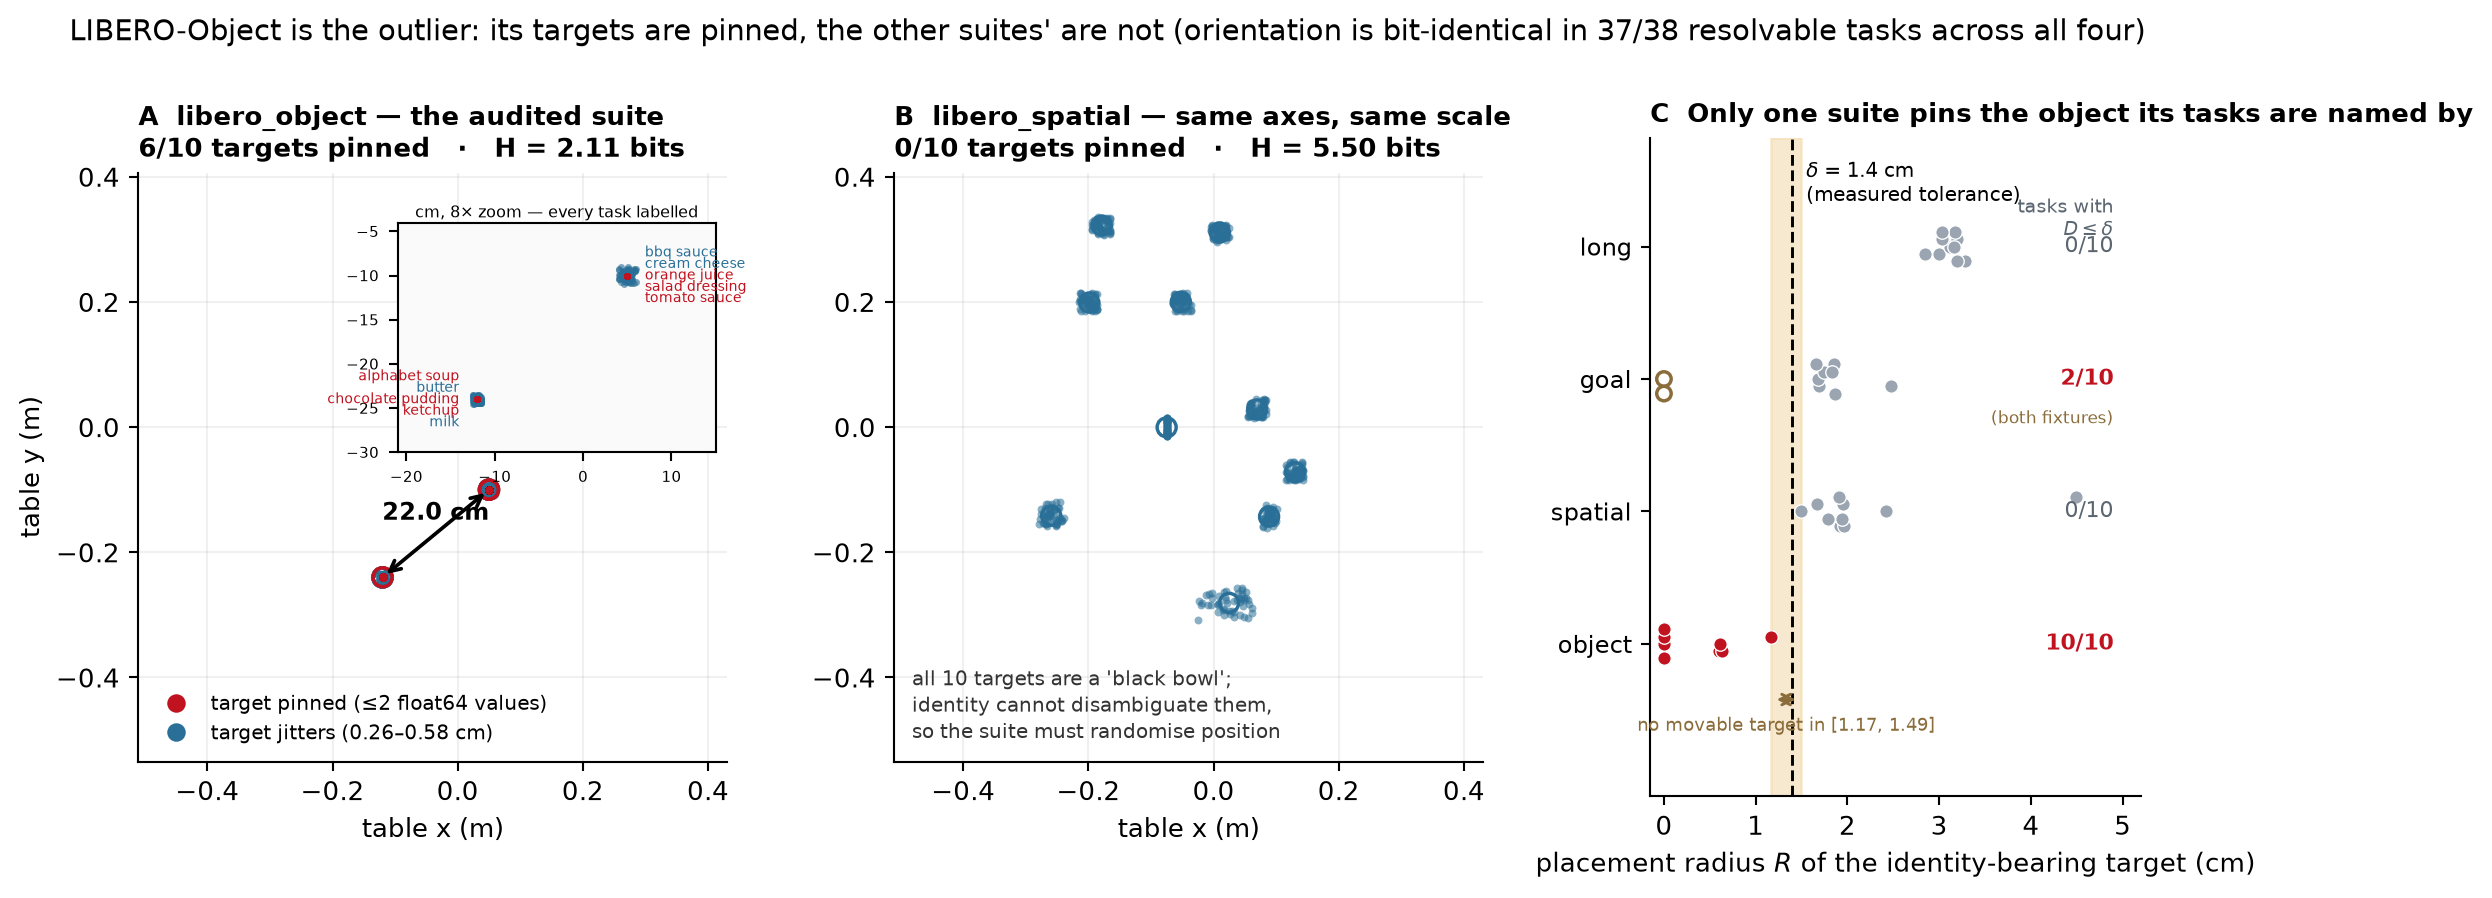
\includegraphics[width=0.98\linewidth]{../visuals/F1_placement_forensics.png}
\caption{Placement forensics. \textbf{A} LIBERO-Object's identity-bearing
targets, $10$ tasks $\times$ $50$ shipped states; six collapse to a point and
the ten task means occupy two clusters $22.1$\,cm apart. \textbf{B}
LIBERO-Spatial on identical axes: every target scatters, and it must, because
all ten of its targets are a ``black bowl'' and identity cannot disambiguate
them. \textbf{C} placement radius per task against the tolerance measured for
this controller. Generated by
\texttt{paper/render\_fig1\_placement\_forensics.py}; SHA-256 digests of every
init-state array are in \texttt{results/suite\_forensics\_columns.json}.}
\label{fig:forensics}
\end{figure*}

Table~\ref{tab:suites} is the measurement, and it says one thing precisely.

\begin{quote}
\textbf{On the object that individuates its tasks, LIBERO-Object is
lookup-admissible on all ten. Among the other thirty tasks, two are --- and
both are fixtures that never move at all.}
\end{quote}

\noindent The threshold is not doing the work. LIBERO-Object's largest
identity radius is $1.171$\,cm; the smallest among the other suites' twenty-eight
\emph{movable} targets is $1.492$\,cm. Every $\delta$ in that gap returns the
same verdict, and the radius we measure for this controller
($\approx 1.41$\,cm, \S\ref{sec:refute}) falls inside it. That is the one
coincidence in this paper that went our way, and we note it is a coincidence:
had the measured radius come out at $2$\,cm, LIBERO-Goal would be $10/10$ too.

\paragraph{How pinned is pinned.} In $6$ of Object's $10$ tasks the target's
start position takes exactly \emph{two} \texttt{float64} values, one unit in the
last place apart on a single axis --- constant to the precision the format can
express. The other four have $R \in [1.17, 1.19]$\,cm.

Across tasks the structure is tighter still: the ten targets occupy two table
positions $22.1$\,cm apart, five tasks each (Figure~\ref{fig:forensics}A), so a
two-constant table covers the identity-bearing half of the whole suite.

\paragraph{This is a property of the shipped files, not of the task
definition.} The BDDL for task $0$ declares a $5 \times 5$\,cm sampling region
for the alphabet soup. The fifty shipped states place it at one point. So the
pinning is an artifact of state generation, not of benchmark design --- which
makes it cheap to fix, and is the strongest argument in this paper for
re-sampling rather than redesigning.

\paragraph{What we do not claim.} That a low radius \emph{causes} a policy to
memorise; that any published policy exploits it; or that admissibility on the
identity-bearing object is sufficient for a constant to solve a task.
\S\ref{sec:refute} shows the last of those failing on our own stack, decisively.

\section{A glass-box stack}
\label{sec:platform}

The artifact is an instrument, not a contribution. It is built to be traceable
end to end, and its size ($30.2$\,M deployed) is what makes an end-to-end trace
feasible rather than a claim about efficiency.

\begin{table}[h]\centering\footnotesize
\setlength{\tabcolsep}{3.5pt}
\begin{tabular}{lrll}
\toprule
component & params & trained & deployed \\
\midrule
YOLO-World-S detector & 13.0\,M & never & frozen \\
world model (TRM) & 9.97\,M & stage A & frozen, inert$^\dagger$ \\
trunk heads & 7.0\,M & stage A & frozen \\
goal heads $+$ gates & 0.24\,M & stage B & frozen \\
\midrule
\textbf{deployed} & \textbf{30.2\,M} & 17.2\,M trained & all frozen \\
\bottomrule
\end{tabular}
\caption{Parameter ledger. There is \emph{no} language model: the
open-vocabulary detector's own text tower supplies every text embedding, so one
frozen network is the only vision encoder \emph{and} the only text encoder.
$^\dagger$Inert in the one cell we have ablated: a persistence baseline
reproduces the held-out cell exactly. We state it for that cell only.}
\label{tab:ledger}
\end{table}

Text is parsed into source/target phrases; the detector is prompted with them
and returns a source box. A grasp head maps
$(\text{uv}, \text{conf}, \text{proprio}, \text{box\_emb}, \text{frame\_emb})$
to a world grasp point --- note the absence of any text argument, which is
Figure~\ref{fig:dataflow}'s point and \S\ref{sec:cert}'s architectural evidence.
A place head maps the command embedding to a place $(x,y)$, latched once per
episode inside \texttt{reset()} and never re-read. A non-learned state machine
converts goals into servo commands within a $\pm6$\,cm probe envelope.

\paragraph{Three words, used throughout.}
\begin{itemize}\itemsep1pt \parskip0pt \topsep2pt \leftmargin0pt
\item \textbf{cell} --- one evaluation: a fixed (head, flags, seed, $n$) run to
completion, always quoted with its $n$ and its interval.
\item \textbf{band} --- the set of shipped initial states a cell replays. The
harness fixes it; it is not sampled.
\item \textbf{burned} --- a band we have looked at and let influence a choice.
From that moment it no longer measures generalisation, and no amount of
re-running un-burns it.
\end{itemize}

\paragraph{Protocol.} LIBERO at commit \texttt{8f1084e3}, MuJoCo $2.3.7$,
robosuite $1.4.1$, torch $2.8.0$, ultralytics $8.4.115$, numpy $2.2.6$,
Python $3.10$, \texttt{MUJOCO\_GL=osmesa} --- \S\ref{sec:cert} explains why
that last entry is not boilerplate.

Which states compose a cell is derivable from its command line, not logged.
The harness sets $\texttt{trial\_seed} = \texttt{seed}\cdot 1{,}000{,}003 +
\texttt{trial}$ and indexes state $\texttt{trial\_seed} \bmod 50$; since
$1{,}000{,}003 \equiv 3 \pmod{50}$, trial $i$ at seed $s$ replays state
$(3s+i) \bmod 50$:

\begin{table}[h]\centering\small
\begin{tabular}{lll}
\toprule
cell & seed, $n$ & states \\
\midrule
dev & 0, 10 & 0--9 \\
held-out & 20, 10 & 10--19 \\
held-out $n{=}50$ & 20, 50 & \textbf{0--49} \\
untouched & 40, 30 & \textbf{20--49} \\
\bottomrule
\end{tabular}
\caption{Which of the $50$ shipped initial states composes each evaluation
cell, derived from the harness's seeding rule rather than logged. Because
$\texttt{trial\_seed} = \texttt{seed}\cdot 1{,}000{,}003 + \texttt{trial}$ and
$1{,}000{,}003 \equiv 3 \pmod{50}$, trial $i$ at seed $s$ replays state
$(3s+i) \bmod 50$. The bolded rows are the ones that matter: an $n{=}50$ cell
is the entire state set and therefore \emph{contains} the dev and held-out
bands rather than being disjoint from them.}
\label{tab:bands}
\end{table}

\noindent The answer is not flattering: \textbf{the $n{=}50$ cells are not
disjoint from the dev and held-out bands --- they contain them.} Fifty trials over fifty shipped states is
the whole set. The untouched band exists to supply one clean cell, and
\S\ref{sec:repairs} reports it.

\section{Executing the proposition}
\label{sec:constant}

Proposition~\ref{prop:lookup} describes a policy. This section runs it, on the
one task where our stack works at all, and \S\ref{sec:refute} runs it on the
other nine --- where it refutes the reading we had given it.

The vehicle is our own stack (\S\ref{sec:platform}): a learned goal head that
emits a world grasp point, driving a non-learned pick-and-place controller.
That factorisation is what makes the experiment clean --- we replace the
\emph{goal supply} and change nothing else. Figure~\ref{fig:ladder}B lists the
five arms and what each may read. Two need a word. \textbf{random} draws from
the observed extent of the scene's objects, re-drawn per episode --- the
controller's floor. \textbf{reset-oracle} reads the true position \emph{once}
at reset and holds it; on a task with $R=0$ that is numerically a per-task
constant, but it still reads the simulator, so it is \textbf{not}
Proposition~\ref{prop:lookup}'s policy.

\begin{figure*}[t]\centering
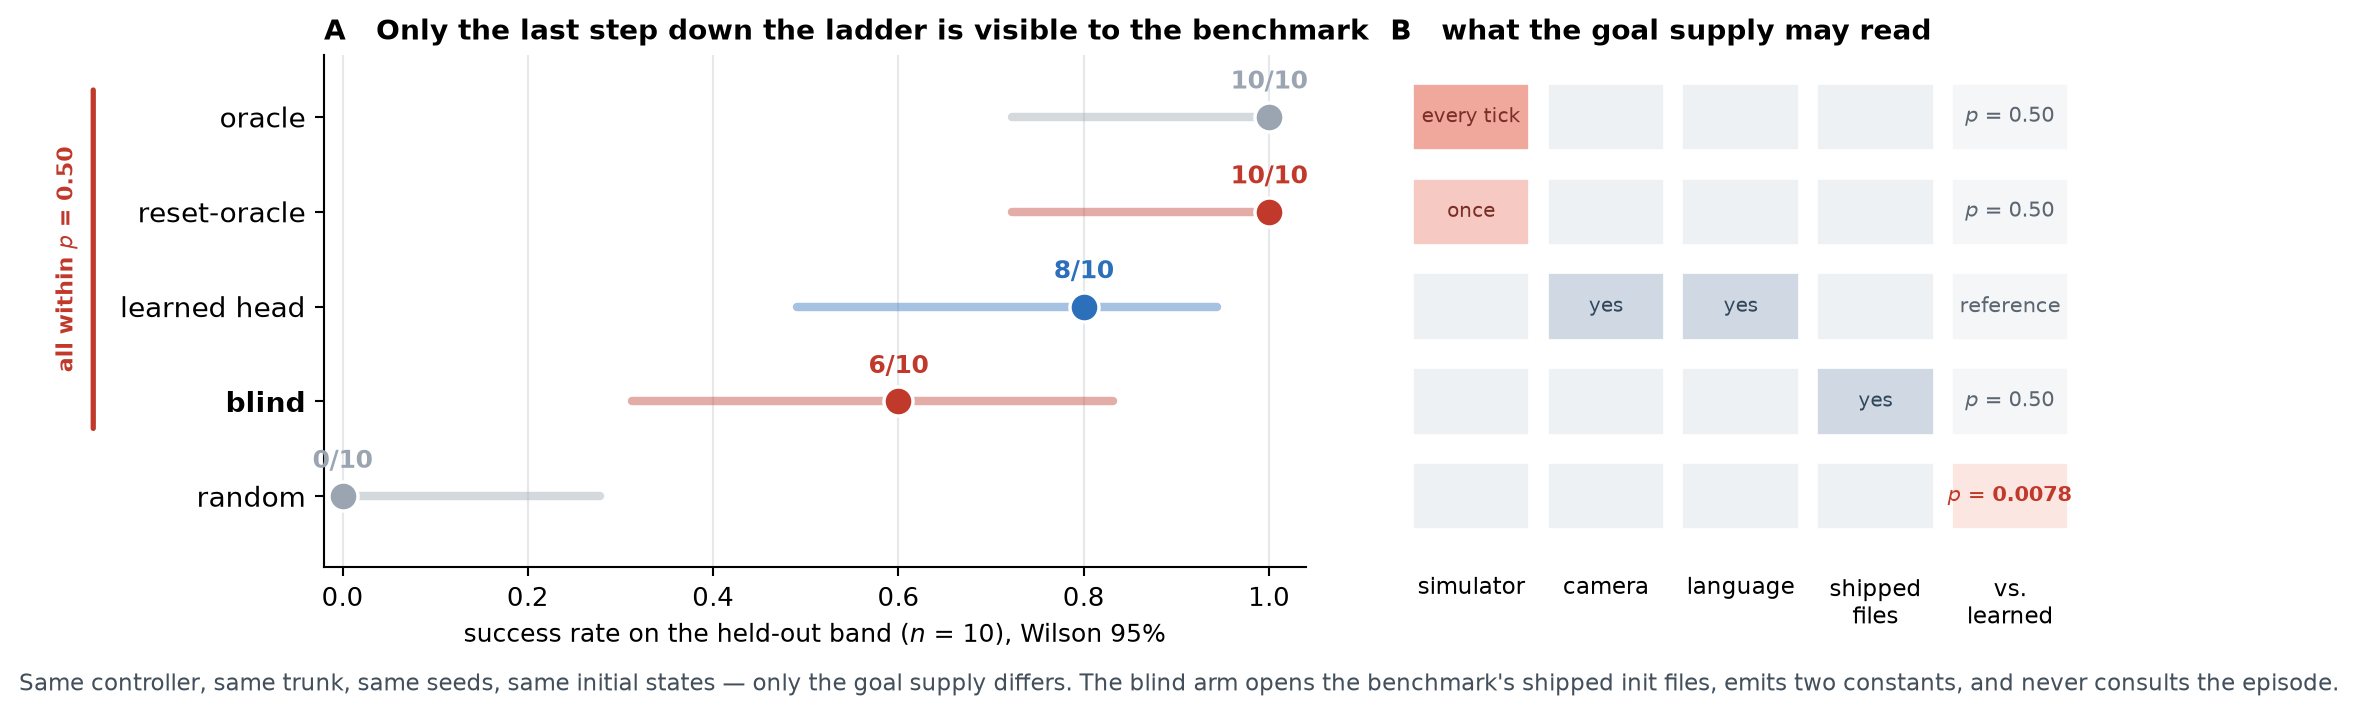
\includegraphics[width=0.97\linewidth]{../visuals/F7_ladder.png}
\caption{\textbf{The goal-supply ladder}, on task $0$. Five arms, one
controller, one trunk, one protocol, one set of initial states; the only
difference is where the goal comes from. \textbf{B} is the experiment:
descending the ladder removes information. \textbf{A} is the result --- and the
honest reading of it is that at $n{=}10$ this cell resolves almost nothing. The
bracket marks arms the cell fails to separate, which is a statement about its
power, not a finding of equivalence. Artifacts:
\texttt{results/pod\_cells.json}, \texttt{results/blind\_cells.json}.}
\label{fig:ladder}
\end{figure*}

\paragraph{The floor is zero.} With an uninformed goal the machinery scores
$0/10$ $[0.00, 0.28]$: eight discordant pairs, all favouring the learned head,
exact McNemar $p = 0.0078$. \textbf{The controller cannot do this task without
a goal.} That is the control that makes the rest of the section mean anything.

\paragraph{The strictly-blind policy.} The \textbf{blind} arm takes the task
index, opens the shipped initial-state files, and emits two constants --- the
mean shipped position of the identity-bearing object and of the container. On
task $0$ those are $(-0.1200, -0.2400, 0.0150)$ and $(0.0023, 0.2605)$.

On this task the grasp constant is not an approximation of the target position;
it \emph{is} the target position. All fifty shipped states place the alphabet
soup at a single $(x,y)$ --- the fifty rows reduce to one --- so whatever the
blind arm fails at, it cannot be error in where it thinks the object is.

\textbf{It scores $6/10$} $[0.31, 0.83]$, against the released head's $8/10$.
We report no inference from that pair. At $n{=}10$ an exact paired test with
two discordant pairs returns $p = 0.50$, which is the largest value the test
can return with any discordance at all; a power calculation gives $0.058$
against the observed effect. \textbf{The cell resolves nothing, and an earlier
version of this paper reported it as though it resolved indistinguishability.}
It does not, and the corollary does not rescue it: Corollary~\ref{cor:sep}
quantifies over policies accurate everywhere, and an $8/100$ policy is not one.

Three honest caveats on the arm itself, none of which we found and all of which
survived into a previous draft. The constant is the \emph{mean} over all fifty
shipped states, which contains the ten this cell replays --- it is fitted, very
weakly, on its own test set. The arm reads the object's identity from the live
scene's body registry rather than from the task index, so ``reads only the task
index'' overstates it. And it requires a live simulator to start at all. The
\emph{control} claim survives all three --- with an anchor set, the goal machine
is driven by proprioception and the constant, and the grasp head is never
called --- but the \emph{blindness} claim as we first wrote it did not.

\section{The whole suite, and a refutation of our own reading}
\label{sec:refute}

\begin{figure*}[t]\centering
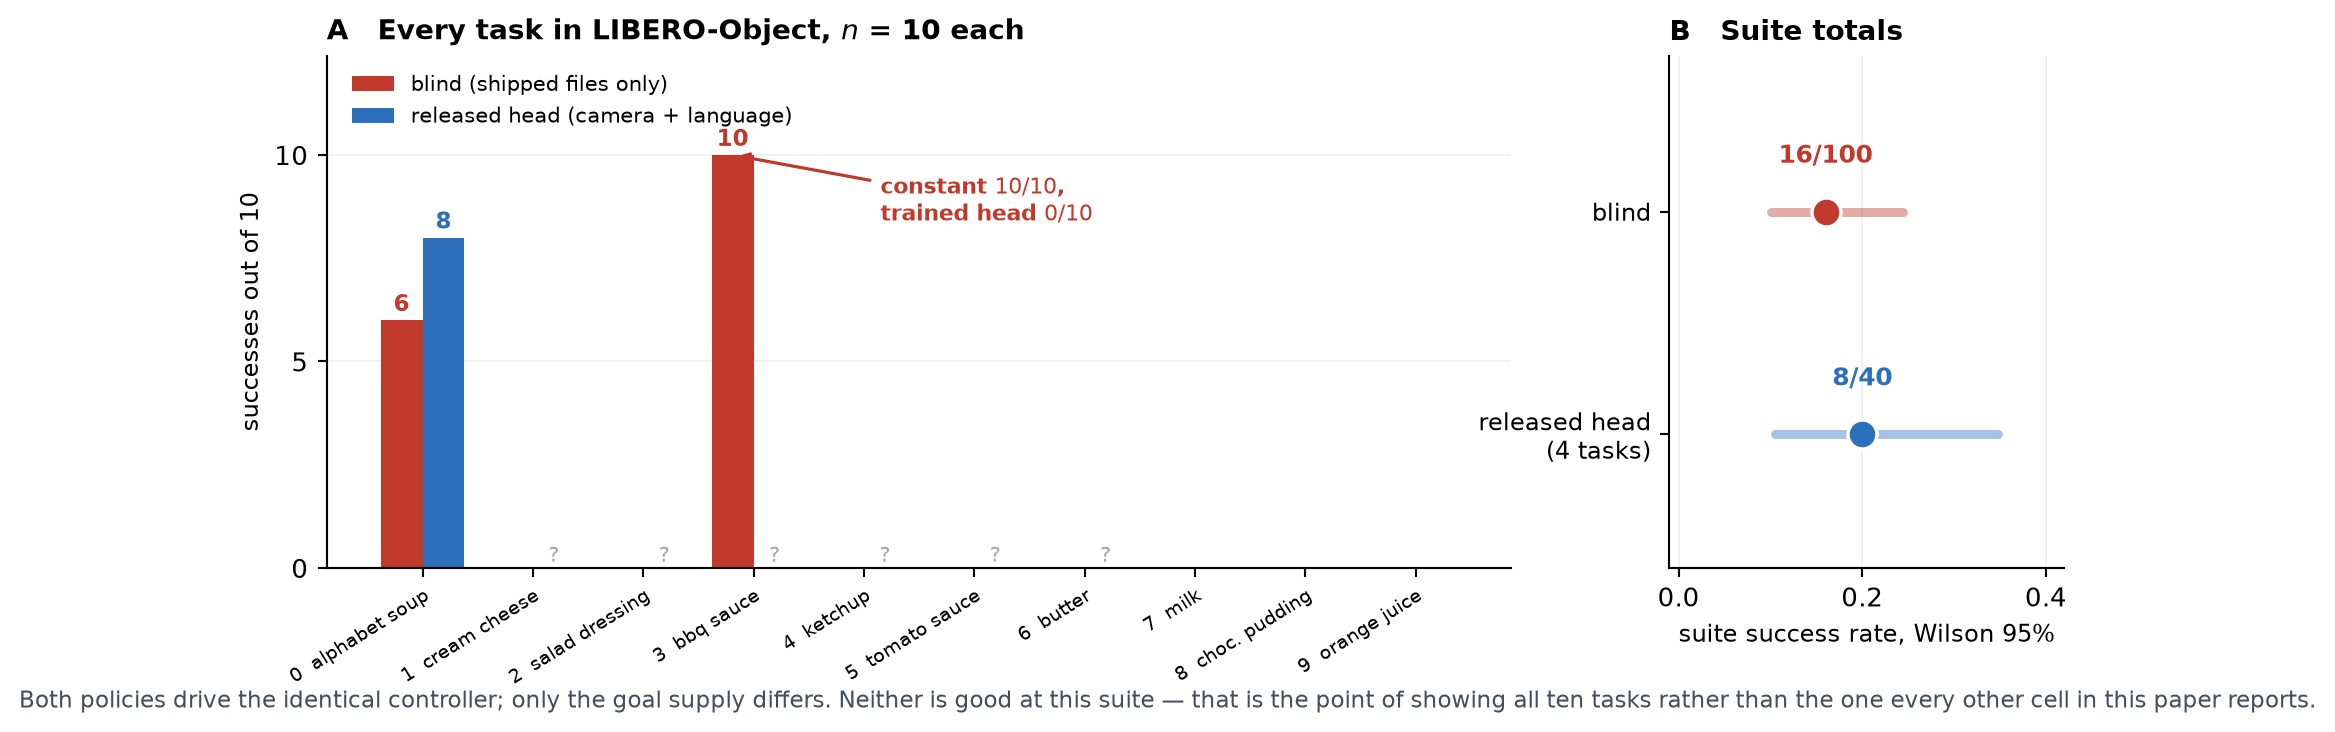
\includegraphics[width=0.97\linewidth]{../visuals/F9_suite.png}
\caption{\textbf{All ten LIBERO-Object tasks}, $n{=}10$ each, every trial
recorded; both policies drive the identical controller. Eight of ten tasks are
$0$--$0$. The suite totals in \textbf{B} are shown with i.i.d.\ Wilson
intervals, which are \emph{too narrow} here by a design effect of $8.4$
(\S\ref{sec:refute}); they are drawn as reported rather than as believed.
Artifacts: \texttt{results/suite\_cells.json},
\texttt{results/suite\_inference.json}.}
\label{fig:suite}
\end{figure*}

Every cell above is one task. Run on all ten, the blind constant scores
$16/100$ and the released head $8/100$. An earlier version of this paper led
with that pair, paired the $100$ trials, ran an exact McNemar, obtained
$p = 0.039$, and concluded that a task-indexed constant significantly beats a
trained vision-language policy.

\textbf{That inference is wrong, and the error is instructive.}

\paragraph{The unit of analysis.} All twelve discordant pairs live in two of
ten tasks, and ten of them in one (Table~\ref{tab:fullsuite}). Within that task
the ten ``trials'' are near-identical replays: blind terminates at steps
$210$--$214$ (sd $1.08$), the head runs to the $300$ cap on all ten. They are
one deterministic contrast counted ten times. At the task level --- the unit
the design actually randomises over --- blind wins one task, loses one, and ties
eight: exact sign test $p = 1.0$, exact sign-flip permutation $p = 1.0$,
cluster bootstrap on the difference $[-0.06, +0.30]$. The design effect is
$8.4$, so the effective $n$ is about $12$, not $100$.

\begin{table}[h]\centering\footnotesize
\setlength{\tabcolsep}{4pt}
\begin{tabular}{llll}
\toprule
unit & test & result & \\
\midrule
trial ($n{=}100$) & exact McNemar & $10$--$2$, $p = 0.039$ & \emph{invalid} \\
task ($n{=}10$) & exact sign & $1$--$1$, 8 ties, $p = 1.0$ & valid \\
task ($n{=}10$) & permutation & $p = 1.0$ & valid \\
task ($n{=}10$) & cluster bootstrap & $[-0.06, +0.30]$ & valid \\
\bottomrule
\end{tabular}
\caption{The same comparison at two units of analysis. Trials within a task
share an object, a scene, a goal supply and a near-deterministic trajectory, so
the trial-level test is anti-conservative by a design effect of $8.4$.
\textbf{There is no suite-level difference between the two policies at the
unit this design randomises over.} Artifact:
\texttt{results/suite\_inference.json}.}
\label{tab:fullsuite}
\end{table}

\paragraph{The constant is not what produced the successes.} This is the
sharper finding, and it comes from the same run.

If the blind arm's score came from the constant being close to the truth, tasks
handed the \emph{same} constant would score alike. Table~\ref{tab:attrib} shows
they do not. The ten tasks fall into two groups by table position; within each,
the constants agree to under a millimetre; and within each, the scores range
from $0$ to $10$.

\begin{table}[h]\centering\footnotesize
\setlength{\tabcolsep}{4pt}
\begin{tabular}{llr}
\toprule
tasks & constants agree to & blind scores \\
\midrule
$0, 4, 6, 7, 8$ & $0.95$\,mm & $6, 0, 0, 0, 0$ \\
$1, 2, 3, 5, 9$ & $0.63$\,mm & $0, 0, \mathbf{10}, 0, 0$ \\
\bottomrule
\end{tabular}
\caption{\textbf{The goal supply does not explain the outcome.} Tasks whose
constants are identical to within a millimetre score anywhere from $0/10$ to
$10/10$. Tasks given a \emph{bit-exact} constant ($R=0$) score $6/60$; tasks
given the loosest constants ($R > 1$\,cm) score $10/40$. The correlation
between placement radius and success is $r = +0.52$, where
Proposition~\ref{prop:lookup} requires it to be non-positive. Artifact:
\texttt{results/constant\_attribution.json}.}
\label{tab:attrib}
\end{table}

What varies across those tasks is the object, not the number. So the blind
arm's two non-zero cells are evidence that \emph{this controller can grasp two
of ten groceries}, and not evidence about lookup. \textbf{We withdraw the
suite-level claim.}

\paragraph{Where A1 does break, we can see it.} One place in this data does
behave the way the proposition expects. On task $0$ the blind arm reaches the
object to within $2$\,mm on all ten trials --- the grasp constant is exact
there --- and the four failures are the four trials whose \emph{basket} sits
furthest from the constant, occupying ranks $6$, $8$, $9$ and $10$ of ten
(exact Mann-Whitney $p = 0.019$, Figure~\ref{fig:subgoal}). Task $3$ tolerates
$1.91$\,cm and never fails. That gives the $\approx 1.4$\,cm radius
\S\ref{sec:adm} uses, and shows it is task-dependent.

Two caveats we owe a reader, because this is the number \S\ref{sec:adm} leans
on. The hypothesis was formed \emph{after} a pre-registered one failed, on the
same ten points. And the covariate is confounded with trial order: the outcome
is exactly $\mathbf{1}\{\text{trial} \le 5\}$, trial $i$ replays state $10+i$,
and displacement correlates with state index at $\rho = 0.65$, so trial index
alone predicts better ($p = 0.0095$). At $n{=}10$ the design cannot separate
them.

\begin{figure*}[t]\centering
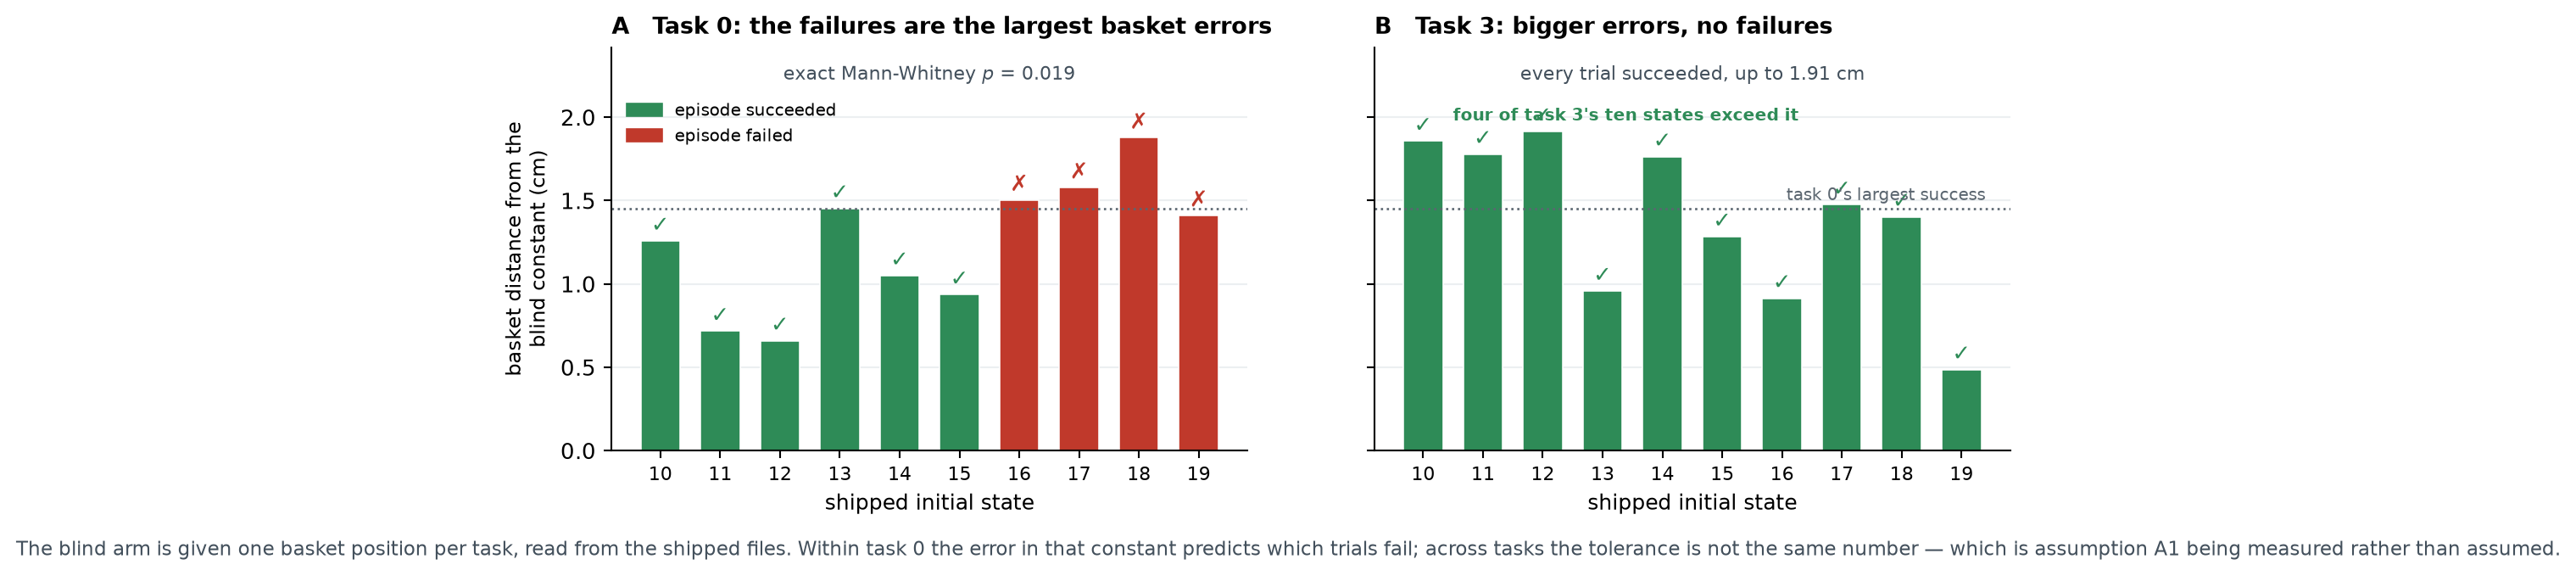
\includegraphics[width=0.97\linewidth]{../visuals/F8_subgoal.png}
\caption{\textbf{The one place the constant demonstrably matters.}
\textbf{A} On task $0$, the trials that fail are those whose basket sits
furthest from the single constant the blind arm was handed. \textbf{B} On task
$3$ the same quantity runs higher and every trial succeeds, so the tolerance is
not one number across tasks. This is the measurement \S\ref{sec:adm}'s
$\delta \approx 1.4$\,cm comes from; see the confound caveats in the text.
Artifact: \texttt{results/blind\_failure\_attribution.json}.}
\label{fig:subgoal}
\end{figure*}

\paragraph{What would settle it.} Displace the constant by $r$ and sweep $r$:
if the score is flat in $r$, the arm never used the number. We implemented it
(\texttt{-{}-goal-anchor-jitter-cm}) and the compute window closed before it
ran. Until it does, the strongest statement the suite supports is the negative
one above.

\paragraph{What survives.} Two things, and we think they are the more useful
two. First, on task $3$ a constant scores $10/10$ where the trained head scores
$0/10$ --- a single task-level event, so we quote no $p$ for it, but a striking
one: the head is not merely worse there, it never succeeds. Second, and
independent of any of this, \textbf{eight successes in a hundred trials, every
one on the single object the head was trained for}. Our artifact is a
one-object solution that a suite-level score would have reported as a policy.
The number a reader should carry away is not $0.700$; it is $0.700$ on task $0$,
with $0.000$ next to it nine times.

\paragraph{And it bounds the audit in advance.} Whatever
\S\ref{sec:audit}--\S\ref{sec:repairs} bought, it was not a general policy. We
put this section before the audit so that no reader reaches the repairs holding
a larger idea of the artifact than the artifact supports.

\section{The audit: four layers}
\label{sec:audit}

``The policy memorised the location'' is not one hypothesis but four, at four
stages --- causal confusion~\citep{dehaan2019causal} spread across a pipeline
rather than confined to a network --- two of which are not in the model at all --- and those two are the ones
a black-box perturbation study cannot reach (Figure~\ref{fig:threat}).

\begin{figure*}[t]\centering
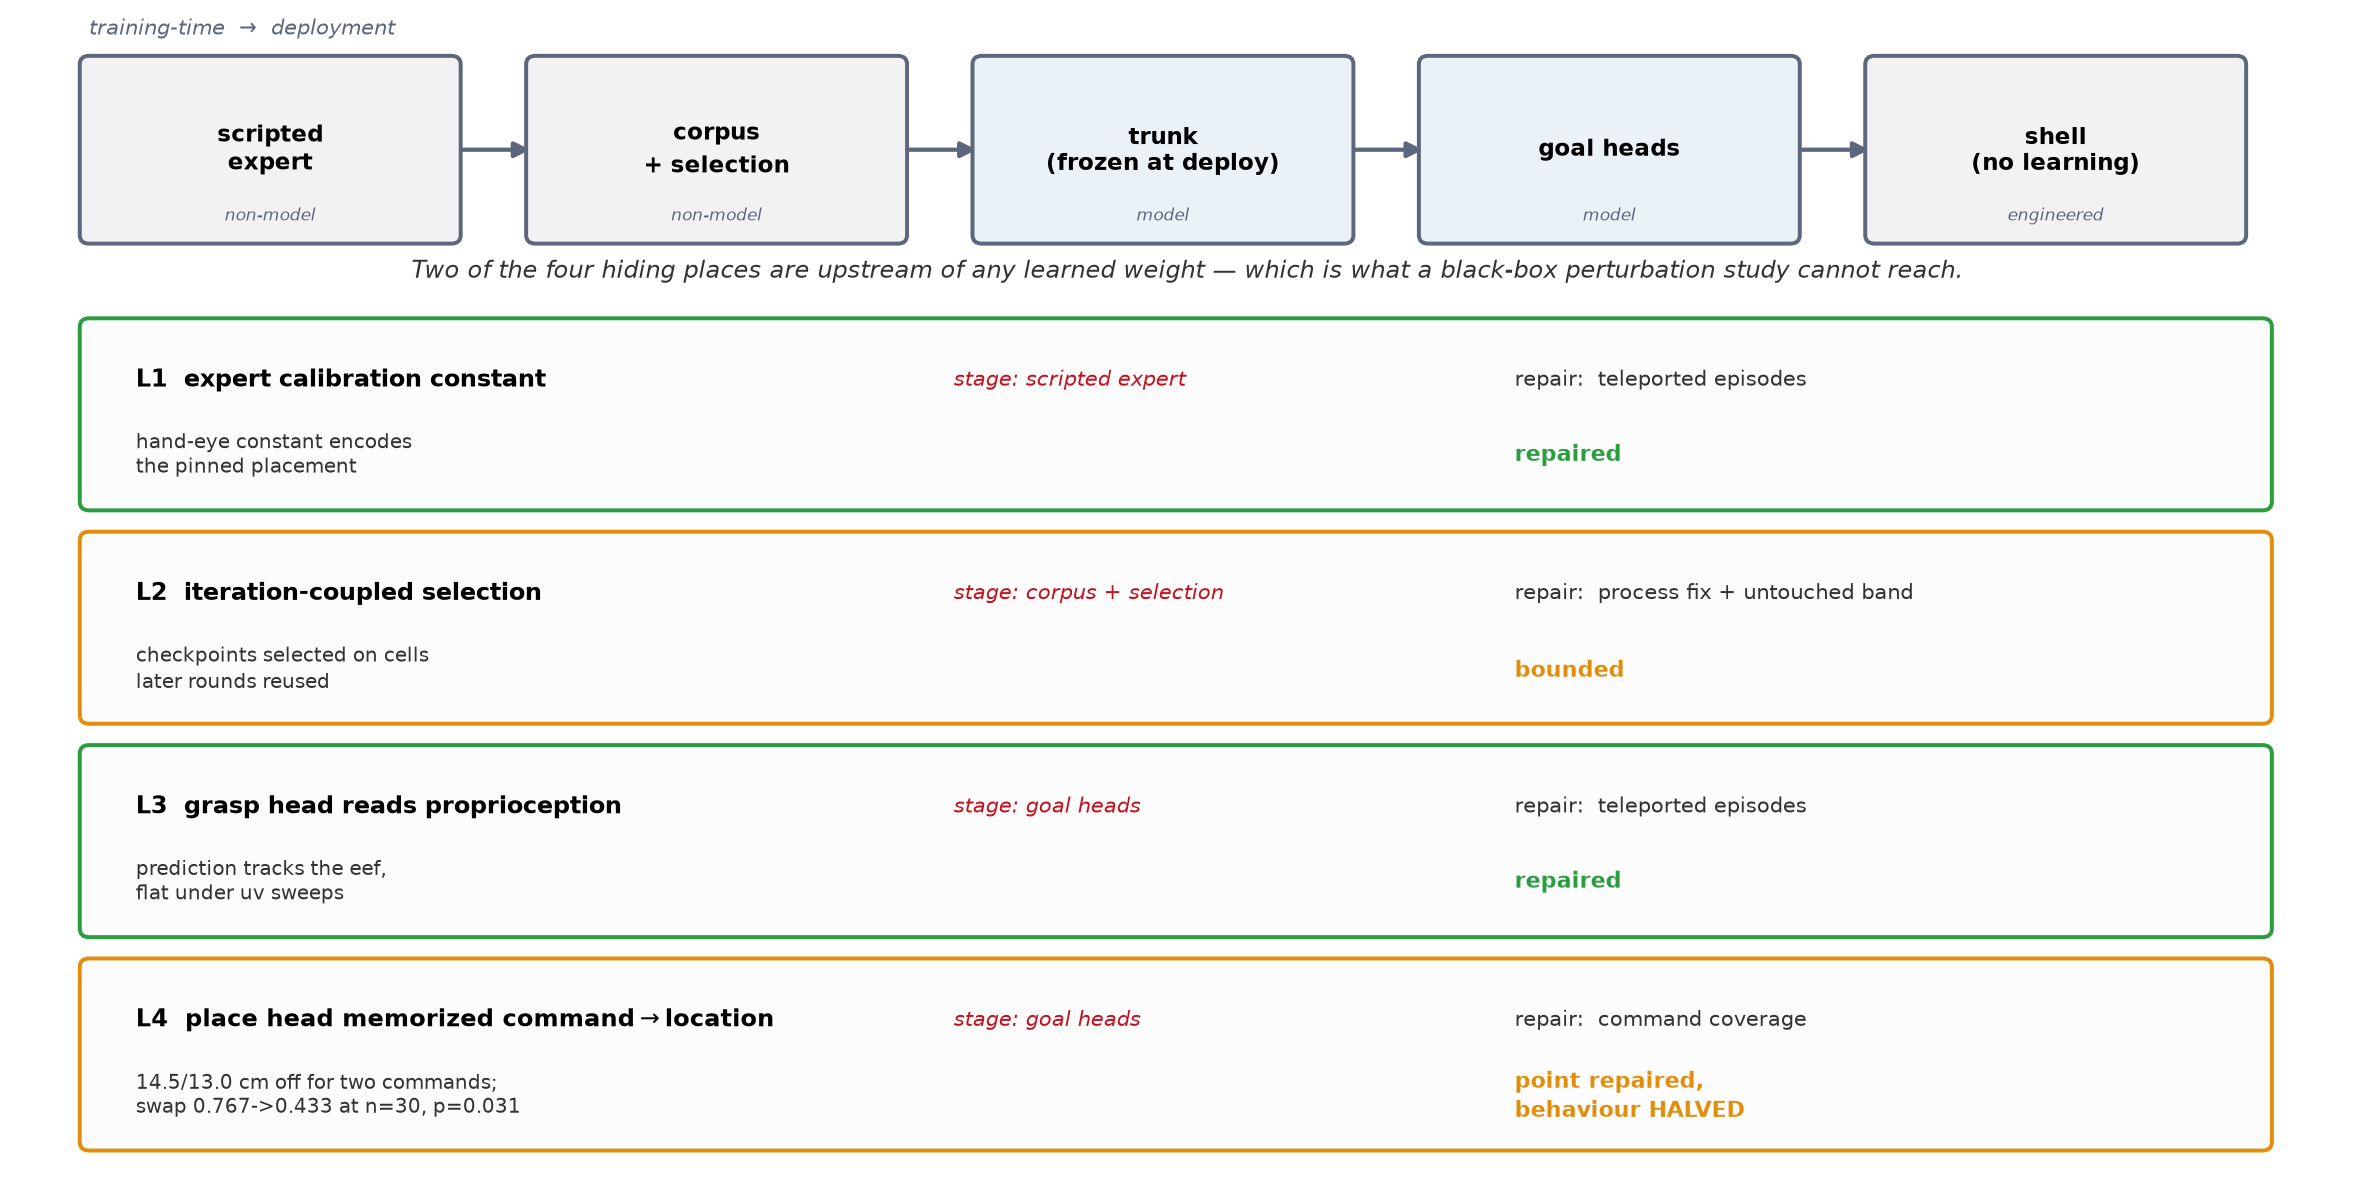
\includegraphics[width=0.98\linewidth]{../visuals/F3_threat_model.png}
\caption{Where a fixed placement can hide in one stack, and the status of each
site. Two of the four sit upstream of any learned weight.}
\label{fig:threat}
\end{figure*}

\begin{table*}[t]\centering\small
\setlength{\tabcolsep}{4pt}
\begin{tabular}{p{1.9cm}p{2.2cm}p{4.2cm}p{2.6cm}p{4.2cm}}
\toprule
layer & where & evidence & repair & verification / status \\
\midrule
1. expert calibration constant & scripted expert (non-model) &
hand-eye constant encodes the pinned placement &
placement teleportation &
$0/10 \to 7/10$ dev, paired. \textbf{Repaired} \\
\addlinespace
2. selection loop & our own procedure (non-model) &
checkpoints chosen on cells later rounds reused &
process fix; bands frozen &
untouched band $20/30$ vs $0.700$: no detected inflation.
\textbf{Bounded, not removed} \\
\addlinespace
3. grasp-head proprio. & \texttt{GraspPointHead} &
prediction tracks the eef, flat under uv sweeps &
same teleported episodes &
attribution flips to visual. \textbf{Repaired} \\
\addlinespace
4. place-head cmd$\to$location & \texttt{PlaceHead} &
correct basket for the trained command, $14.5$/$13.0$\,cm off for the other
two; swap $8/10 \to \mathbf{0/20}$, $p{=}0.0078$ &
command coverage &
place \emph{point} $14.15 \to 0.78$\,cm \textbf{repaired}; swap
\emph{behaviour} $0.767 \to 0.433$, $p{=}0.031$ --- \textbf{halved, not fixed} \\
\midrule
\emph{(separate)} appearance drift & deployment viewpoints &
NN-cosine gap on the policy's own trajectory &
DAgger on own viewpoints &
$3/50 \to 22/50$ vs $3/50$ control, $p<10^{-4}$. \textbf{Repaired} \\
\bottomrule
\end{tabular}
\caption{Master audit table. Layers 1--4 are the placement-memorisation layers;
the last row is a drift case study, \emph{not} one of the four; it appears here
only because its repair is easily mistaken for one of theirs. Two rows are
deliberately not marked repaired.}
\label{tab:audit}
\end{table*}

Three of the four are described here; the fourth, being the one the instruments
found rather than confirmed, gets its own subsection.

\paragraph{Layer 1: the expert's calibration constant.} The scripted
demonstrator carried a hand-eye offset fitted once, on a scene whose target
never moved. That constant therefore \emph{encoded} the pinned placement, and
every demonstration inherited it --- so the corpus taught the pose before any
network saw a pixel. Detected by reading the expert, not the policy. Repaired by
re-baking ten episodes with the source object displaced, which breaks the
constant's validity and forces the demonstrator to look; the repaired corpus
lifts the dev cell from $0/10$ to $7/10$ on the same episodes.

\paragraph{Layer 2: the selection loop.} Our own procedure, not the artifact's:
at each round we chose a checkpoint using cells that later rounds reused, so
selection pressure accumulated on one band of initial states. This is invisible
to any measurement of the model and is the reason \S\ref{sec:repairs} runs an
untouched band at all. It is \emph{bounded} rather than repaired --- one cannot
un-look at data --- and the bound is that thirty never-inspected states score
within noise of the burned ones.

\paragraph{Layer 3: the grasp head's proprioceptive shortcut.} Substitution
attribution showed the predicted grasp point tracking the end-effector and
barely moving under $uv$ substitution: the head had learned to predict where the
object is from where the arm is, which on a pinned suite is a sufficient
statistic. The same teleported episodes repair it, and the released head's
profile inverts --- it now moves further on its visual channels
($3.43$/$6.57$\,cm) than on proprioception ($1.93$\,cm).

\subsection{Layer 4: where the language goes}
\label{sec:language}

\begin{figure*}[t]\centering
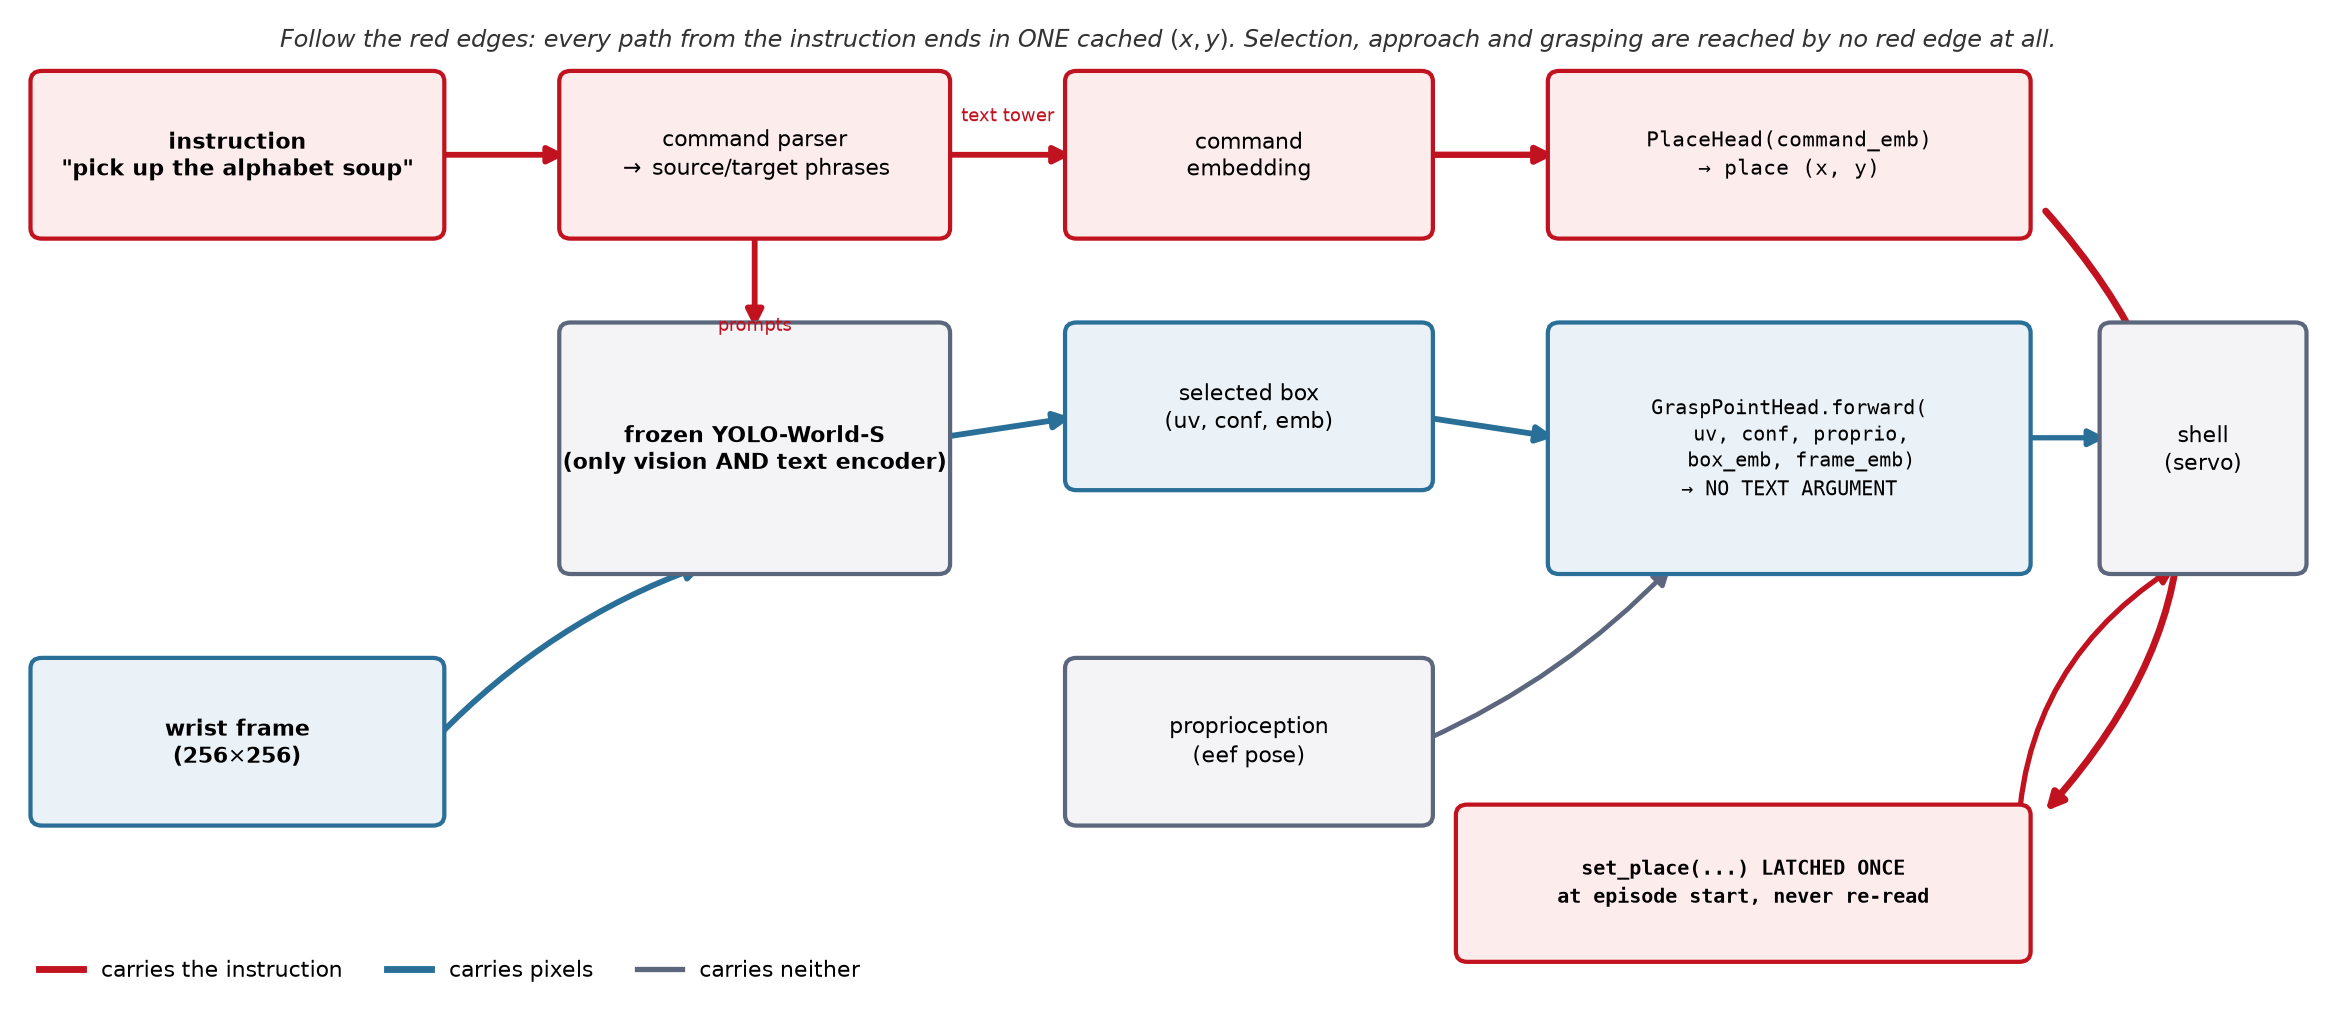
\includegraphics[width=0.98\linewidth]{../visuals/F2_dataflow_language.png}
\caption{Every edge coloured by what it carries. The architectural half of the
argument is a code fact: \texttt{GraspPointHead.forward} takes no text argument,
so no red edge reaches object selection, approach or grasping, and every red
edge terminates in one $(x,y)$ latched once per episode and never re-read.}
\label{fig:dataflow}
\end{figure*}

Swapping the instruction while holding the scene and the success predicate fixed
collapses the released head from $8/10$ to $\mathbf{0/20}$ $[0.00,0.16]$; on the
ten trials that pair with the reference cell, eight discordant pairs all one way,
exact McNemar $p = 0.0078$.

Telemetry places the failure \emph{downstream of approach}: the policy still
reaches the true object as closely as baseline while the grip-close rate falls
from ${\sim}0.67$ to ${\sim}0.26$. Driving the detection prompts and the
place-head embedding from \emph{different} instructions isolates the collapse to
one channel, with no interaction.

Combined with the architecture: \textbf{object selection, approach and grasping run with
no language input at all, and the entire language channel is a single cached
$(x,y)$}. Ask this policy for the butter and it finds, approaches and grasps the
alphabet soup at baseline rate; it fails only when that one coordinate is wrong.

\begin{figure*}[t]\centering
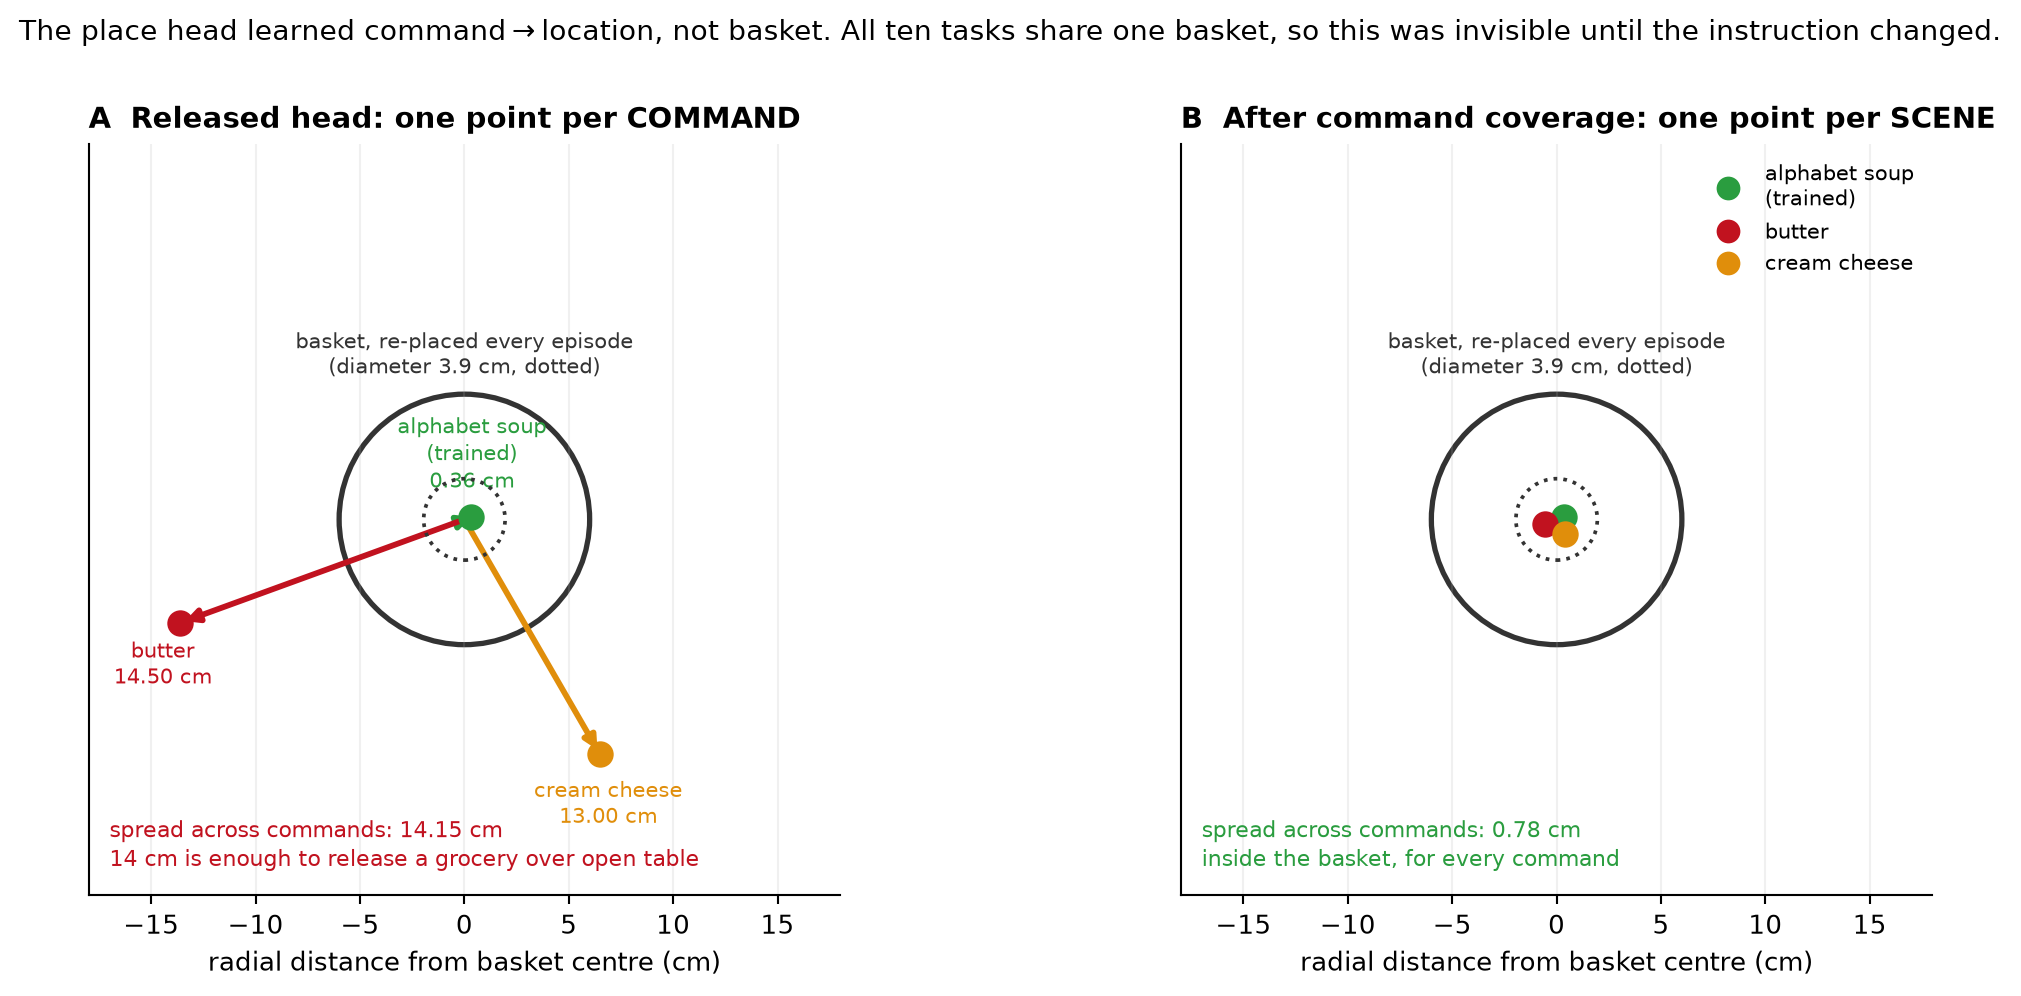
\includegraphics[width=0.92\linewidth]{../visuals/F6_place_point_map.png}
\caption{Layer 4 drawn rather than argued. The released head asked for three
objects emits three place points, $14.5$ and $13.0$\,cm from the basket. The
basket itself is \emph{not} fixed --- it is re-placed every episode, with a
per-task diameter of $3.66$\,cm (max $3.96$) --- so a memorised place point is wrong by
$14$\,cm against a target that only ever moves by $4$, and $14$\,cm is enough
to release a grocery over open table. Radial distances are measured; angles are for
legibility.}
\label{fig:placepoint}
\end{figure*}

\section{Repairs, and one we withdraw}
\label{sec:repairs}

Three of the four layers admit a repair, and we report what each bought. One
claim from the previous version does not survive being run at power, and we
retract it here rather than leave it standing.

\paragraph{The untouched band.} Both $n{=}50$ cells contain the burned states,
so we ran the released head on states $20$--$49$, which no selection look ever
reached, with the prediction recorded before the run ($[0.50,0.75]$, falsifiers
named in both directions). Result: $\mathbf{20/30 = 0.667}$ $[0.49,0.81]$,
against the published $0.700$ ($35/50$) a difference of $-0.033$, Newcombe
$[-0.24,+0.16]$. That interval assumes independent samples and the samples are
\emph{not} independent: the $n{=}50$ cell spans states $0$--$49$ and so contains
all thirty untouched states.

The interval is therefore conservative in the wrong direction, and we use it
only to bound the effect as small. The clean comparison --- untouched-$30$
against the twenty genuinely burned states --- is the one we would run next.

We claim exactly this much: not that the burn is zero, but that it is small
enough to hide inside $\pm 0.20$, which is what $n{=}30$ buys.

\paragraph{A repair we withdraw.} Command coverage was reported as repairing
the instruction-swap behaviour on the strength of $3/10$ against a $4/10$
baseline at $p = 1.0$. That is an equivalence claim from an underpowered cell,
on a band where the head was already mostly failing --- and a swap cannot
visibly break a cell that is already broken. Re-run on a band where the coverage
head scores well, and taken to $n{=}30$:

\begin{table}[h]\centering\small
\begin{tabular}{llll}
\toprule
head & baseline & swapped & paired McNemar \\
\midrule
released head & 8/10 & \textbf{0/20} & $p=0.0078$ \\
coverage & 23/30 & \textbf{13/30} & $p=0.031$ \\
\bottomrule
\end{tabular}
\caption{Substituting a different task's instruction, on a band where each head
scores well and at a power the original cell did not have. Both heads lose
accuracy, so command coverage does not eliminate the instruction dependence it
was built to remove; it halves it. Paired McNemar over matched trial indices
(same seed, same initial states, same renderer --- only the instruction
differs), exact two-sided.}
\label{tab:swap}
\end{table}

\noindent At $n{=}10$ this contrast was $p=0.125$ and we would have called it
unresolved; at $n{=}30$ it is $p=0.031$. \textbf{The coverage head collapses
too.} A swap cannot visibly break a cell that is already mostly broken, which is
why the original $4/10$ baseline hid the effect.

What replaces the withdrawn claim is more useful than it was. Coverage does not
eliminate the failure, it roughly \emph{halves} it: the released head loses its
entire cell ($0.800 \to 0.000$, every discordant pair one way), the coverage
head about a third ($0.767 \to 0.433$). And the repair to the place
\emph{point} is not in doubt --- $14.15 \to 0.78$\,cm
(Figure~\ref{fig:placepoint}), measured directly rather than inferred from
behaviour.

So: \textbf{command coverage fixes where the head aims and does not fully fix
what it does.} A residual command$\to$location dependence survives training on
all three commands --- a sharper statement of layer 4 than we had, and one no
cell we ran before could have detected.

\subsection{Randomisation is a curve, not a point}
\label{sec:sweep}

Our $\pm4$\,cm radius was chosen to sit inside the controller's $\pm6$\,cm probe
envelope --- a perturbation calibrated to the system under test. Sweeping it on
the same draws separates two things that single number confounded:

\begin{table}[h]\centering\small
\begin{tabular}{lll}
\toprule
displacement & released head & Wilson 95\% \\
\midrule
none & 4/10 & $[0.17,0.69]$ \\
$\pm2$\,cm & 7/10 & $[0.40,0.89]$ \\
$\pm4$\,cm & 4/10 & $[0.17,0.69]$ \\
$\pm6$\,cm (envelope edge) & 2/10 & $[0.06,0.51]$ \\
$\pm8$\,cm (outside) & 3/10 & $[0.11,0.60]$ \\
\bottomrule
\end{tabular}
\caption{Sweeping the placement-randomisation radius on the same draws.
Randomisation robustness is a curve, and at $n{=}10$ this curve is not even
monotone --- the undisplaced cell sits \emph{below} $\pm2$\,cm, which cannot be
a real benefit of displacement. Reporting any single radius as ``passes
randomisation'' would quote a number this sample does not resolve.}
\label{tab:sweep}
\end{table}

\noindent Read conservatively, because $n{=}10$ supports no more: clearly worse
at $\pm6$--$\pm8$ than at $\pm2$, but every interval is ${\sim}0.5$ wide and the
undisplaced cell sits \emph{below} $\pm2$\,cm, which cannot be a real benefit of
displacement. That non-monotonicity is the honest measure of what this $n$
resolves. \textbf{No single radius should be quoted as ``passes
randomisation''}, and a benchmark asking for one is asking for a number that
does not exist.

\section{Certification}
\label{sec:cert}

If a benchmark score cannot certify grounding, what can? This section reports
three results about the certification problem itself, two of them negative.

\subsection{Probes alone cannot certify}

A substitution probe asks which input channels a head reads: swap one channel
between two recorded ticks and measure how far the predicted grasp offset moves.
It is annotation-free, cheap, and on-manifold --- and that last property is
fatal on its own.

\begin{figure*}[t]\centering
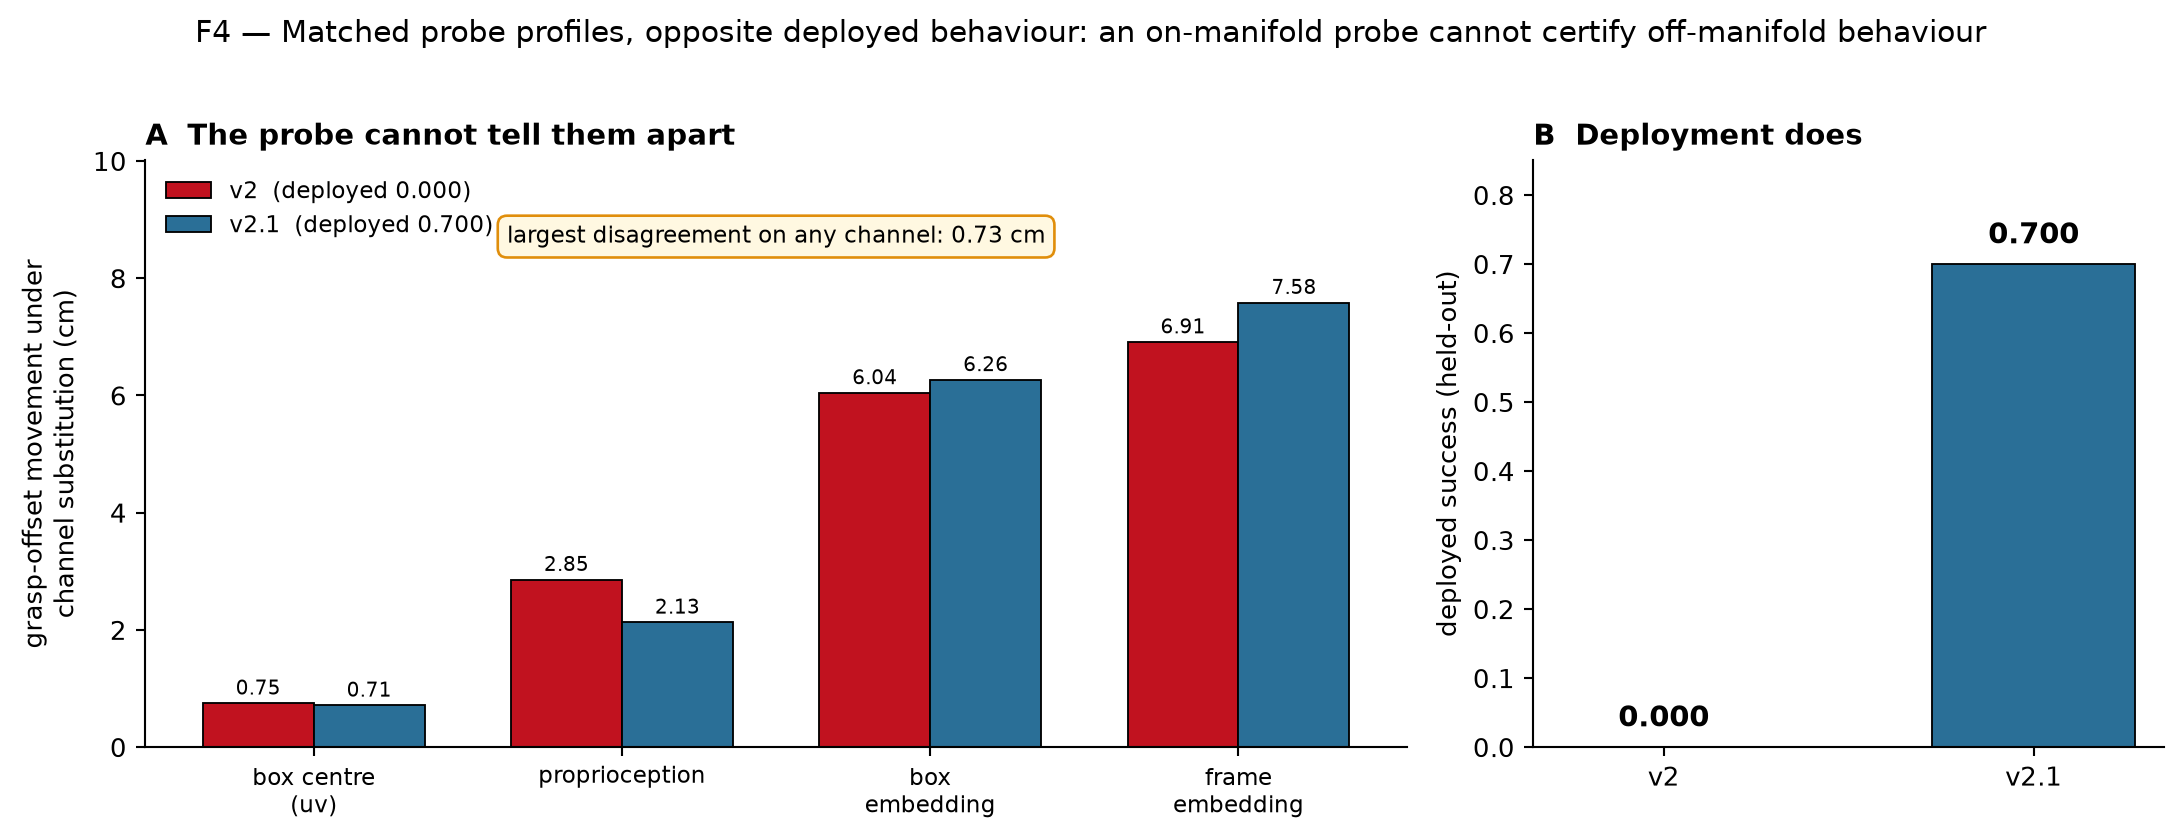
\includegraphics[width=0.9\linewidth]{../visuals/F4_probe_counterexample.png}
\caption{Two heads trained the same way on the same $10$-episode corpus. Their
attribution profiles agree to within $0.73$\,cm on every channel; deployed, they
score $0.000$ and $0.700$. Regenerated by
\texttt{scripts/attribution\_profiles.py}.}
\label{fig:counterexample}
\end{figure*}

\begin{table}[h]\centering\small
\begin{tabular}{lrrrr}
\toprule
head & uv & proprio & box\_emb & frame\_emb \\
\midrule
v2 & 0.75 & 2.85 & 6.04 & 6.91 \\
v2.1 & 0.71 & 2.13 & 6.26 & 7.58 \\
v5 (released) & 0.97 & 1.93 & 3.43 & 6.57 \\
\bottomrule
\end{tabular}
\caption{Substitution-probe attribution, in cm of movement of the predicted
grasp \emph{offset}, per input channel. The counterexample is the first two
rows: v2 and v2.1 agree to within $0.73$\,cm on every channel and score
$0.000$ and $0.700$ when deployed. A probe evaluated on teacher trajectories
cannot, on its own, certify off-manifold behaviour.}
\label{tab:probe}
\end{table}

\noindent One detail in Table~\ref{tab:probe} decides whether the probe means
anything: it profiles the grasp \emph{offset}, not the absolute point. The head
emits $\text{eef}_{xy} + \Delta$, so substituting proprioception moves the
absolute prediction by the entire arm displacement for \emph{any} head, and
profiling that quantity reports ${\sim}24$\,cm of ``proprioception
attribution'' even for a repaired one.

We made exactly this error when regenerating the measurement. We record it
because it is the difference between a probe that answers ``does this channel
change where the head thinks the object is'' and one that measures the
parameterisation.

\textbf{v2 and v2.1 differ by at most $0.73$\,cm on any channel and score
$0.000$ and $0.700$ deployed} (Figure~\ref{fig:counterexample}). One caveat we
state rather than let a reader discover: the substitution is between a
\emph{single} pair of recorded ticks --- the two most separated in $uv$ out of
$329$ --- with no resampling over pairs and therefore no interval on the
$0.73$\,cm. It is an existence proof that two heads can be probe-identical and
behaviourally opposite, not an estimate of how often that happens.

A probe evaluated on teacher trajectories is an on-manifold instrument and
cannot, alone, certify off-manifold behaviour. Probe evidence must be paired
with behavioural randomisation.

\subsection{An instrument only ever shown firing is not yet an instrument}

Our cross-instruction detection-agreement probe asks whether two objects' prompt
chains select the \emph{same box from the same frame}; a high same-box rate says
the grounding stage carries no object identity. Every published number from it
was a firing. Running it against every other object in the scene splits cleanly:

\begin{table}[h]\centering\footnotesize
\setlength{\tabcolsep}{4pt}
\begin{tabular}{lrrl}
\toprule
counterpart & $n$ & same-box & median dist. \\
\midrule
cream cheese, butter, pudding & 6 & \textbf{0.00} & $0.817$--$0.818$ \\
tomato sauce & 4 & 1.00 & $0.00069$ \\
bbq sauce, salad dressing & 5 & $0.80$ & $0.0043$ \\
ketchup & 5 & $0.60$ & $0.0048$ \\
\bottomrule
\end{tabular}
\caption{The positive control our detection-agreement instrument had never been
given. ``Same-box'' is the fraction of frames on which two objects' prompt
chains select the identical box; a high rate means the grounding stage carries
no object identity. Run against \emph{every} counterpart rather than only the
ones that fire, the instrument separates cleanly --- and the split is
interpretable: the chains that collide are the cans and bottles, the ones that
separate are the boxes. Deployed binding is blind \emph{within} a shape class,
which is the regime LIBERO-Object's groceries occupy. Small $n$ (only $4$--$6$
of $60$ frames have both chains detecting) makes these demonstrations of
discrimination, not calibrated rates.}
\label{tab:poscontrol}
\end{table}

\noindent The instrument registers difference when difference exists. The
distances are bimodal --- collisions at ${\sim}0.004$, separations at
${\sim}0.82$, nothing between --- and a sweep over
$\tau \in \{0.005,0.01,0.02,0.05\}$ leaves every verdict unchanged. The split is
interpretable and sharpens the claim: the chains that collide are the cans and
bottles, the ones that separate are the boxes. \textbf{Deployed binding is blind
\emph{within a shape class}}, which is precisely the regime LIBERO-Object's
groceries occupy.

Two limits. Only $4$--$6$ of $60$ frames had both chains detecting, so these are
small-$n$ demonstrations of discrimination, not calibrated rates. And the
contrast we originally designated the positive control --- the basket --- is not
evaluable at all: the deployed source-area filter rejects basket-sized boxes by
construction, so it compares zero frames. Our first version of the script read
$\text{same\_rate}=0$ off that empty comparison and printed ``instrument
discriminates''. A verdict now requires $n \ge 3$.

\subsection{Certificates are joint in (head, stack), down to the renderer}

We rebuilt the deployment stack on fresh hardware, pinning every version in
\S\ref{sec:platform} and verifying both load-bearing checkpoints by
digest. The reference cell reproduces: $8/10$ $[0.49,0.94]$ against a recorded
$7/10$, with $0.700$ inside the interval.

Reproducing the \emph{rate} is not reproducing the \emph{experiment}. Holding
seed, trial, weights and every package version fixed and changing only the
OpenGL backend MuJoCo renders through:

\begin{table}[h]\centering\small
\begin{tabular}{lll}
\toprule
& \texttt{osmesa} & \texttt{egl} \\
\midrule
success rate & 8/10 & 8/10 \\
per-trial outcomes & \multicolumn{2}{l}{\textbf{4 of 10 disagree} (2 each way)} \\
\bottomrule
\end{tabular}
\caption{Changing only the OpenGL backend MuJoCo renders through --- same
seed, same trials, same weights, same package versions. The aggregate is
identical and $40\%$ of the individual episodes are not. Matching a published
rate is therefore weak evidence of having reproduced an experiment, and any
paired statistic computed across a renderer change is invalid, because pairing
assumes the trials are the same trials.}
\label{tab:renderer}
\end{table}

\noindent \textbf{The aggregate is identical and $40\%$ of the episodes are
not.} Thread count, by contrast, changes nothing we could detect: three
\texttt{osmesa} runs at $1$, $4$ and $128$ threads agree on all eight logged
fields while the wall clock falls from $220$\,s to $32$\,s. We state the
limit plainly --- that comparison ran to $40$ steps, a prefix in which the
gripper never closes, so it does not probe the contact-rich part of an
episode where the renderer difference showed up
(\texttt{results/thread\_determinism.json}). Software and GPU
rasterisation do not produce identical pixels, the detector is not invariant to
that difference, and in this stack the detector is the only encoder.

Two consequences. Matching a published rate is weak evidence of having
reproduced an experiment: the marginal can be right while the sample is
different. And \emph{any paired statistic computed across a renderer change is
invalid}, because pairing assumes the trials are the same trials --- every
McNemar in this paper is within one backend, which we can now say we checked
rather than assumed. \texttt{MUJOCO\_GL} belongs in any reported stack; it was
not in ours, or in any LIBERO evaluation we have read.

\section{Transfer: a negative result}
\label{sec:transfer}

The instruments above are offered as portable. We therefore attempted to run
them on a policy we did not build: the public
\texttt{openvla-7b-finetuned-libero-object} checkpoint~\citep{kim2024openvla}, evaluated through the
same harness, the same trial$\to$state map and the same success predicate.

We report a negative, and the discipline that produced it matters more than the
outcome. The baseline returned $0/1$ on a checkpoint published near $0.9$. That
is a harness defect, not a finding about OpenVLA, and we treated it as one.

Four defects were found and fixed: image orientation, the gripper convention (their
model emits $[0,1]$ with $1{=}$close, robosuite wants $[-1,+1]$ with
$-1{=}$close --- without the conversion the jaw never closes and the policy
\emph{cannot} grasp), success extraction (the environment's \texttt{done} flag
also fires on horizon), and a missing signal shield. We then swept four image
orientations $\times$ the $0.9$ centre crop their fine-tuned evaluation applies.

The checkpoint still does not approach the target in any configuration we
tried; the end-effector never closes to within a grasp of it.
\textbf{We therefore report no OpenVLA success numbers, and no distance
statistics either} --- the diagnostic runs that produced them were exploratory,
were not written to a versioned artifact, and we decline to quote figures we
cannot ship. An unvalidated
baseline would make our instruments look powerful for entirely the wrong reason
--- every one of the four defects biased in that same direction --- and that is
the easiest way to fabricate an external-validation result without intending to.

We cannot separate the two live hypotheses: a remaining defect in our harness,
or a checkpoint that does not transfer to a differently-built LIBERO. The second
is exactly what \S\ref{sec:cert} predicts and we decline to claim it, because the
first is not excluded. The harness ships (\texttt{eval/openvla\_eval.py}) so the
question is answerable by someone with the matching build. Until then, the
portability of our instruments is \textbf{unestablished}, and we make no claim that these instruments generalise beyond the stack
they were built on.

\section{Negative results and registries}
\label{sec:neg}

A paper that only reports what worked cannot be checked. This section is the
ledger: what we predicted before running, what failed, which instruments we
retired, and the three ways our own results fooled us.

\paragraph{Pre-registration.} Fourteen predictions are on record with
their outcomes. Five earlier ones, all falsified. Two from the confound test
(\S\ref{sec:confound}). Seven registered for this revision, of which five held
--- the untouched band, the oracle ceiling, the uninformed floor, the
reset-oracle, and the released head's swap --- and two failed: that the coverage
head's swap cell would hold (it does not, $p{=}0.031$) and that the released head
would be at floor once displacement left the controller's envelope ($3/10$, not
$\approx0$).

One result in this paper carries \emph{no} registered prediction: the blind arm
(\S\ref{sec:constant}) was implemented in one compute window and run in the
next, and we did not write down an expected rate before running it. We flag it
rather than reconstruct one after the fact. Its per-trial outcomes were fixed
before we looked at any of them, which is the property that matters for the
paired tests, but it is not pre-registration and we do not present it as such.

\paragraph{Retired instruments.} Quantifying deployed role binding was attempted
six times and abandoned six times, each at a calibration gate written down
before the instrument was trusted: a projected-origin ground truth (rejected ---
the object that succeeds $35/50$ scored $0.111$), its sign-corrected successor
(rejected --- the in-frame filter deletes the close-up target by construction),
three text-tower discrimination probes (rejected --- each failed to detect the
working object's own phrase), and a box-spread metric (rejected --- confounded
by camera motion, and inverted). Deployed binding accuracy is reported as
\textbf{unmeasured}.

\subsection{A confound we had missed}
\label{sec:confound}

Our own analysis of a blocked object was confounded: because the suite's two
placement clusters align with which objects we happened to train on,
``blocked'' and ``$22$\,cm from the training position'' were perfectly
correlated in our design. Tested directly over all ten objects, position
predicts the effect weakly (Spearman $+0.19$, $p{=}0.60$) and \emph{teleporting
each object $22$\,cm shows no directional effect} ($6/10$, exact sign test
$p{=}1.0$, the least informative value the test returns), while detector groundability predicts it ($-0.71$, $p{=}0.027$).
The mechanism is appearance, not position --- position is a nuisance term with
mean $|\Delta| = 0.0066$, which is not zero either.

\paragraph{This does not contradict \S\ref{sec:adm}, and the distinction is
worth stating.} Those sections answer different questions. Placement is what the
suite fails to randomise and therefore what a policy \emph{may exploit}: that is
a property of the benchmark, established from its shipped files, and it is what
layers 1 and 3 were caught doing. Appearance is what limits \emph{transfer to a
new object} once that shortcut is repaired: a property of the frozen detector,
and why the released head works on one object and not on nine
(\S\ref{sec:refute}).

A benchmark can be lookup-admissible and a policy can still fail for an
unrelated reason. Both are true here, neither weakens the other, and what
\emph{would} have been a contradiction --- position explaining both --- is what
the confound test ruled out.

We also report the caveats on this cell rather than only its conclusion. Both
nulls are $n{=}10$, which is the size we decline to accept elsewhere
(\S\ref{sec:repairs}); the groundability predictor and the outcome are two
statistics of the same detector forward pass, so their correlation is closer to
a self-consistency check than to an independent prediction; and $p = 0.027$
across three tests does not survive a Bonferroni correction. The confound is
\emph{disconfirmed as a sufficient explanation}, which is what the design can
support, and not more.

\subsection{Three ways a result fooled us}

Recorded because the failure modes generalise and \emph{none} was caught by a
conventional check --- in all three the instrument was correct and the defect
was elsewhere (Table~\ref{tab:fooled}).

\begin{table}[h]\centering\footnotesize
\setlength{\tabcolsep}{3.5pt}
\begin{tabular}{p{1.75cm}p{2.2cm}p{2.95cm}}
\toprule
what we saw & what it was & the general lesson \\
\midrule
a perfect null: teleport gaps identical to control for all ten objects, to four decimals &
a cached observation --- the renderer returned the \emph{pre}-teleport frame &
implausible cleanliness is a symptom. The script now compares frames across the
intervention and \emph{raises} rather than emitting \\
\addlinespace
a defect count withdrawn as unsupported &
the appendix we could not find existed &
``I could not find it'' is a claim about a search, not about a corpus \\
\addlinespace
$7/7$ against a published $7/10$; we began writing up a failure to reproduce &
a censored sample. The complete cell is $\mathbf{8/10}$ &
successes end episodes early and failures run to the horizon, so any interim
harvest is biased toward successes. \textbf{Verifying the instrument does not
verify the sampling} \\
\bottomrule
\end{tabular}
\caption{Three self-inflicted errors and their repairs. The third is the one we
would most expect others to hit: every check we ran had passed, and the defect
was in \emph{when} we looked. The harvester now reports each cell against its
planned $n$ and refuses to report an incomplete one.}
\label{tab:fooled}
\end{table}

\section{Discussion}

\paragraph{What a score certifies.} On a suite whose placement radius sits
below the embodiment's tolerance, a success rate certifies that the policy can
execute a manipulation \emph{given} a correct target pose --- and nothing
whatever about how it obtained one. That is a statement about what the score
\emph{could} distinguish, and it is exactly as strong as A1.

We are careful here because we already overreached once. Our own cells do not
demonstrate that any policy exploited the degeneracy; \S\ref{sec:refute} shows
they cannot. What the radius buys is a check that runs before training, and a
prediction --- that a suite with small radii admits a cheap solution --- which
\citet{jiang2026benchmarking} confirm on LIBERO with a trained probe where we
did not with a constant.

\paragraph{Shortcuts live in pipelines, not only in models.} Two of our four
layers are outside the network: a scripted expert's calibration constant and our
own checkpoint-selection loop. No amount of perturbing a trained model from the
outside would have found either. This is an argument for glass-box artifacts in
benchmark-validity work, and it is the main reason our stack is small.

\paragraph{Certification is a system property.} Probes cannot certify alone
(two heads, $0.73$\,cm apart, $0.000$ vs $0.700$). Behaviour must be paired with
randomisation. And the certificate is joint in \emph{(head, stack)} down to a
component no requirements file pins: the same weights on the same seeds give the
same rate and a different $40\%$ of episodes under a different renderer.

\paragraph{Limitations.}
\begin{itemize}\itemsep1pt \parskip0pt \topsep2pt
\item One simulator, one benchmark suite, one robot, wrist camera only.
\item Every confirmatory cell is one task and one object at $n \le 30$,
including the blind arm ($n{=}10$). The suite-level claims (\S\ref{sec:adm})
are the ones computed from files and do not have this limit.
\item The held-out band is partially burned; the disclosure is in
\S\ref{sec:platform} and the bound in \S\ref{sec:repairs}.
\item The on-manifold limit of substitution probes is a limit on our own
instruments, not only on others'.
\item Transfer to an external policy is \textbf{unestablished}
(\S\ref{sec:transfer}).
\item $D$ and $H_\delta$ are defined for suites shipping enumerable initial
states, and would need restating for procedurally generated ones.
\end{itemize}


\subsection{Recommendation to benchmark authors}

Both quantities are cheap to compute and cheap to report.
Table~\ref{tab:recs} is what we would ask of a suite.

\begin{table}[h]\centering\footnotesize
\setlength{\tabcolsep}{3.5pt}
\begin{tabular}{p{1.6cm}p{2.35cm}p{3.2cm}}
\toprule
practice & cost & why \\
\midrule
publish $D$ and $H_\delta$ per task & one script, no training & tells a reader what a score can certify \\
\addlinespace
set a floor on $D$ & re-sample the init files & a suite individuated by identity must randomise placement, or identity is never load-bearing \\
\addlinespace
ship a tier of radii & $k$ extra eval configs & where a policy degrades depends on displacement relative to the controller's envelope (Table~\ref{tab:sweep}); one radius is a calibration, not a result \\
\bottomrule
\end{tabular}
\caption{Three practices, in increasing order of what they cost a benchmark's
authors. LIBERO-Spatial already satisfies the second by necessity --- all ten
of its targets are the same bowl --- and LIBERO-Object could satisfy it by
choice.}
\label{tab:recs}
\end{table}

\section{Conclusion}

A manipulation benchmark score is not a measurement of capability until the
benchmark's admissibility has been measured. The measurement is cheap, it runs
before any model is trained, and on LIBERO it says something specific: the one
suite whose tasks are individuated by object identity is also the one that pins
that object, on all ten tasks, to a radius smaller than the tolerance we
measure for our own arm.

The behavioural claim we built on that does not stand, and the way it fell is
the more useful half of this paper. We ran the lookup policy, saw it outscore
our trained one, tested it at the wrong unit of analysis, and reported a
significance that a task-level test does not support. The deeper error was
attributional: tasks handed constants identical to within a millimetre score
from $0/10$ to $10/10$, so the successes were never evidence about lookup at
all. Both errors were found by adversarial review of a manuscript we already
believed, using data we had already published.

What survives is the procedure rather than the artifact: measure the benchmark
first, at the unit the design randomises over; check that the variable you
manipulated is the one that moved; and report the reading that did not survive
being checked, which in this revision is our own.

\appendix

\section{Recovering which column owns which object}
\label{app:columns}

LIBERO ships each task's initial states as a MuJoCo flattened state
$[\,t \mid q \mid \dot q\,]$; every shipped $\dot q$ is zero, so the columns
that vary across states are exactly the position degrees of freedom the suite
randomises. Recovering \emph{which} object owns which column requires care. The
fixed layout $[\,t \mid 9 \mid N\!\times\!7 \mid \dot q\,]$ that works for
LIBERO-Object predicts a width of $19+13N$ and fails for every suite containing
an articulated fixture --- LIBERO-Spatial ships width $92$ against $5$ declared
objects. We therefore run two passes: the fixed-layout one, and one that
compiles each task's model and reads \texttt{jnt\_qposadr} with the joint names,
mapping every column onto a named body. \textbf{The two agree wherever both
apply}, and only the second is used for suites the first cannot parse.
Artifacts: \texttt{results/suite\_forensics\_columns.json} (digests),
\texttt{results/suite\_forensics\_joints.json} (per-object positions).

\section{The norm}
\label{sec:norm}

Definition~\ref{def:D} uses the Euclidean norm. A1 is naturally stated in
$\ell_\infty$, because LIBERO randomises placement in an axis-aligned box, and
the two differ by up to $\sqrt{2}$ in the plane. Recomputing
Table~\ref{tab:suites} under $\ell_\infty$ at $\delta = 1.4$\,cm leaves
LIBERO-Object at $10/10$ and moves one LIBERO-Spatial task across the line
($1/10$ instead of $0/10$). The comparison is unchanged; the exact count in one
suite is not. We report the Euclidean version throughout and flag the
dependence here rather than leaving a reader to find it.

\section{Sensitivity of $H_\delta$ to the tolerance}
\label{app:delta}

The quantisation $\delta$ is a modelling choice, so the finding must not depend
on it. Recomputing placement entropy across five tolerances spanning two orders of
magnitude:

\begin{table}[h]\centering\small
\begin{tabular}{lrrrrr}
\toprule
suite & $0.5$mm & $2$mm & $5$mm & $1$cm & $5$cm \\
\midrule
\textbf{Object} & \textbf{2.11} & \textbf{0.48} & \textbf{0.00} & \textbf{0.00} & 0.00 \\
Spatial & 5.48 & 4.49 & 2.04 & 0.25 & 0.00 \\
Goal & 5.59 & 5.08 & 1.53 & 0.02 & 0.00 \\
Long & 5.63 & 5.40 & 4.27 & 0.37 & 0.00 \\
\bottomrule
\end{tabular}
\caption{Mean placement entropy $H_\delta$ in bits, swept over an order of
magnitude in the tolerance $\delta$. LIBERO-Object is lowest at every
tolerance, so the ordering does not depend on the modelling choice --- but
every suite reaches zero by $\delta = 5$\,cm, which is a statement about coarse
resolution rather than about LIBERO. That degeneracy is why the paper's claim
is licensed on the diameter $D$ (Table~\ref{tab:suites}), which has no such
parameter. Artifact: \texttt{results/placement\_entropy.json}.}
\label{tab:deltasweep}
\end{table}

\noindent The ordering is unchanged wherever the measure discriminates at all.
Coarsening $\delta$ lowers every suite's entropy, as it must --- coarser radii
merge components --- and by $\delta = 5$\,cm every suite reaches zero, which is
a statement about coarse resolution rather than about LIBERO. This is precisely
why the paper's claim is licensed on the diameter $D$
(Table~\ref{tab:suites}), which has no such parameter: at
$\delta = 5$\,cm every suite would look admissible on $H$, while on $D$ only
LIBERO-Object is, at any tolerance the controller actually has. Artifact:
\texttt{results/placement\_entropy.json}.

\bibliographystyle{plainnat}
\bibliography{refs}

\end{document}
